% !TeX spellcheck = en_US
% !TeX root = DynELA.tex
%
% LaTeX source file of DynELA FEM Code
%
% (c) by Olivier Pantalé 2020
%
\chapter{DynELA single element sample cases}

\startcontents[chapters]
\printmyminitoc[1]\LETTRINE{T}his chapter deals with some numerical applications of
the \DynELA~for dynamic applications in 2D, axi-symmetric and 3D
cases. In the subsequent tests, if not specified, a Johnson-Cook constitutive
law is used to model the behavior of the material. The Johnson-Cook
hardening flow law is probably the most widely used flow law for the
simulation of high strain rate deformation processes taking into account
plastic strain, plastic strain rate and temperature effects. Since
a lot of efforts have been made in the past to identify the constitutive
flow law parameters for many materials, it is implemented in numerous
Finite Element codes such as Abaqus \cite{abaqus20146}. The general
formulation of the Johnson-Cook law $\sigma^{y}(\overline{\varepsilon}^{p},\stackrel{\bullet}{\overline{\varepsilon}^{p}},T)$
is given by the following equation:

\begin{equation}
\sigma^{y}=\left(A+B\overline{\varepsilon}^{p^{n}}\right)\left[1+C\ln\left(\frac{\stackrel{\bullet}{\overline{\varepsilon}^{p}}}{\stackrel{\bullet}{\overline{\varepsilon}_{0}}}\right)\right]\left[1-\left(\frac{T-T_{0}}{T_{m}-T_{0}}\right)^{m}\right]\label{eq:Samples!Johnson-Cook}
\end{equation}
where $\stackrel{\bullet}{\overline{\varepsilon}_{0}}$ is the reference
strain rate, $T_{0}$ and $T_{m}$ are the reference temperature and
the melting temperature of the material respectively and $A$, $B$,
$C$, $n$ and $m$ are the five constitutive flow law parameters.
A 42CrMo4 steel following the Johnson-Cook behavior law has been selected
for all those tests, and material properties are reported in Table
\ref{tab:Samples!JohnsonCookParameters}.

\begin{table}[h]
\begin{center}\begin{tcolorbox}[width=.75\textwidth,myTab,tabularx={C|C|C|C|C|C|C}]
$E$ & $\nu$ & $A$ & $B$ & $C$ & $n$ & $m$ \\
\small{($Gpa$)} &  & \small{($MPa$)} & \small{($MPa$)} &  &  & \\ \hline
$206.9$ & $0.3$ & $806$ & $614$ & $0.0089$ & $0.168$ & $1.1$ \\ \hline\hline
$\rho$ & $\lambda$ & $C_{p}$ & $\eta$ & $\stackrel{\bullet}{\overline{\varepsilon}_{0}}$ & $T_{0}$ & $T_{m}$ \\
\small{$(kg/m^{3})$} & \small{$(W/m^{\circ}C)$} & \small{$(J/Kg^{\circ}C)$} & & \small{$(s^{-1})$} & \small{$(^{\circ}C)$} & \small{$(^{\circ}C)$} \\ \hline
$7830$ & $34.0$ & $460$ & $0.9$ & $1.0$ & $20$ & $1540$
\end{tcolorbox}\end{center}

\caption{Material parameters of the Johnson-Cook behavior for the numerical
tests\label{tab:Samples!JohnsonCookParameters}}
\end{table}


\section{Uniaxial tensile tests}

\subsection{Element plane tensile test}

The uniaxial one element tensile test is a numerical test where an
plane element (with a square prescribed shape) is subjected to pure
tensile as presented in figure \ref{fig:Samples!Single!Tensile}.
\begin{figure}[h]
\begin{centering}
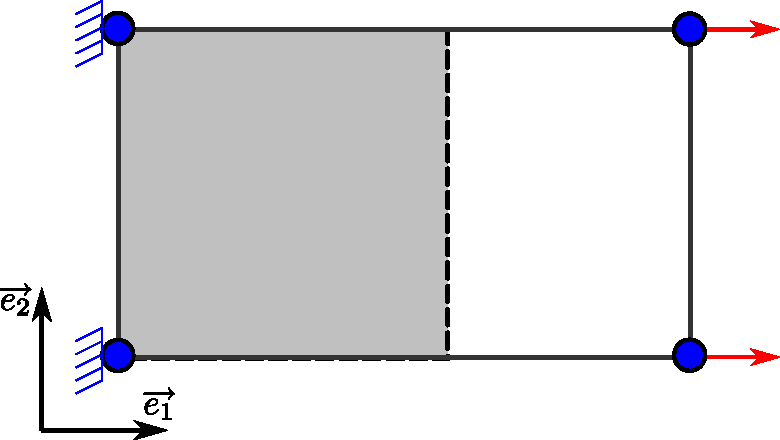
\includegraphics[width=0.5\columnwidth]{Figures/SamplesSingleTensile}
\par\end{centering}
\caption{Numerical model for the one element tensile test\label{fig:Samples!Single!Tensile}}
\end{figure}
 The initial shape of the specimen is $10\,mm\times10\,mm$, the two
left nodes of the element are encastred and a prescribed horizontal
displacement $d=10\,mm$ is applied on the two right nodes of the
same element as illustrated in Figure \ref{fig:Samples!Single!Tensile}.
As we are using an explicit integration scheme, the total simulation
time is set to $t=0.01\,s$.

All the properties of the constitutive law reported in Table \ref{tab:Samples!JohnsonCookParameters}
are used and the material is assumed to follow the Johnson-Cook behavior
described by equation \ref{eq:Samples!Johnson-Cook}.

Figure \ref{fig:Samples!Single!Tensile-Comparison} shows the comparison
of the DynELA solver results (plotted in red) and the Abaqus numerical
results (plotted in blue) concerning the evolution of the stress components
$\sigma_{11}$, $\sigma_{22}$, $\sigma_{12}$, $\overline{\sigma}$,
$\overline{\varepsilon}^{p}$ and $T$ \versus  the horizontal displacement
of the right edge of the specimen along the horizontal axis. For the
Abaqus model, the exact same mesh has been used. Comparison of Abaqus
and DynELA results is made by averaging the DynELA results on the
$4$ integration points of the element. This has been done because
\DynELA~uses full integrated elements while Abaqus have reduced
integrated elements only but in fact, the DynELA results at the $4$
integration points are the same in this benchmark test.

\begin{figure}[h]
\begin{centering}
\begin{tabular}{cc}
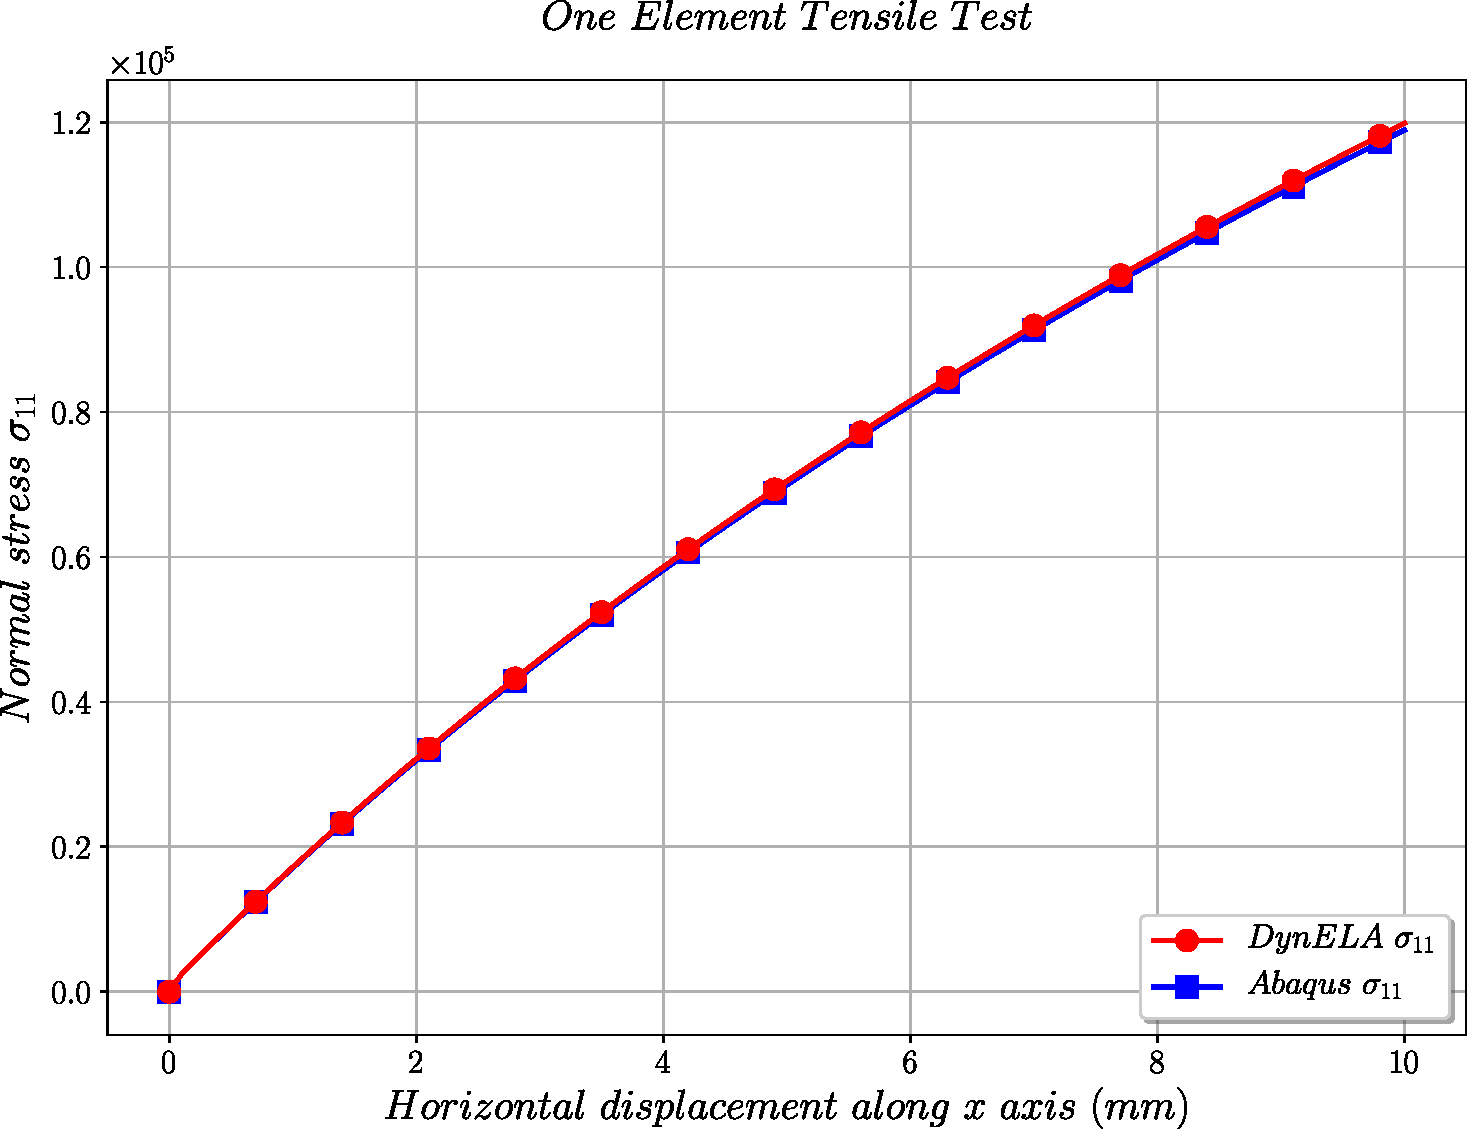
\includegraphics[width=0.45\columnwidth]{Figures/Samples/Element/Tensile_stress_11} & 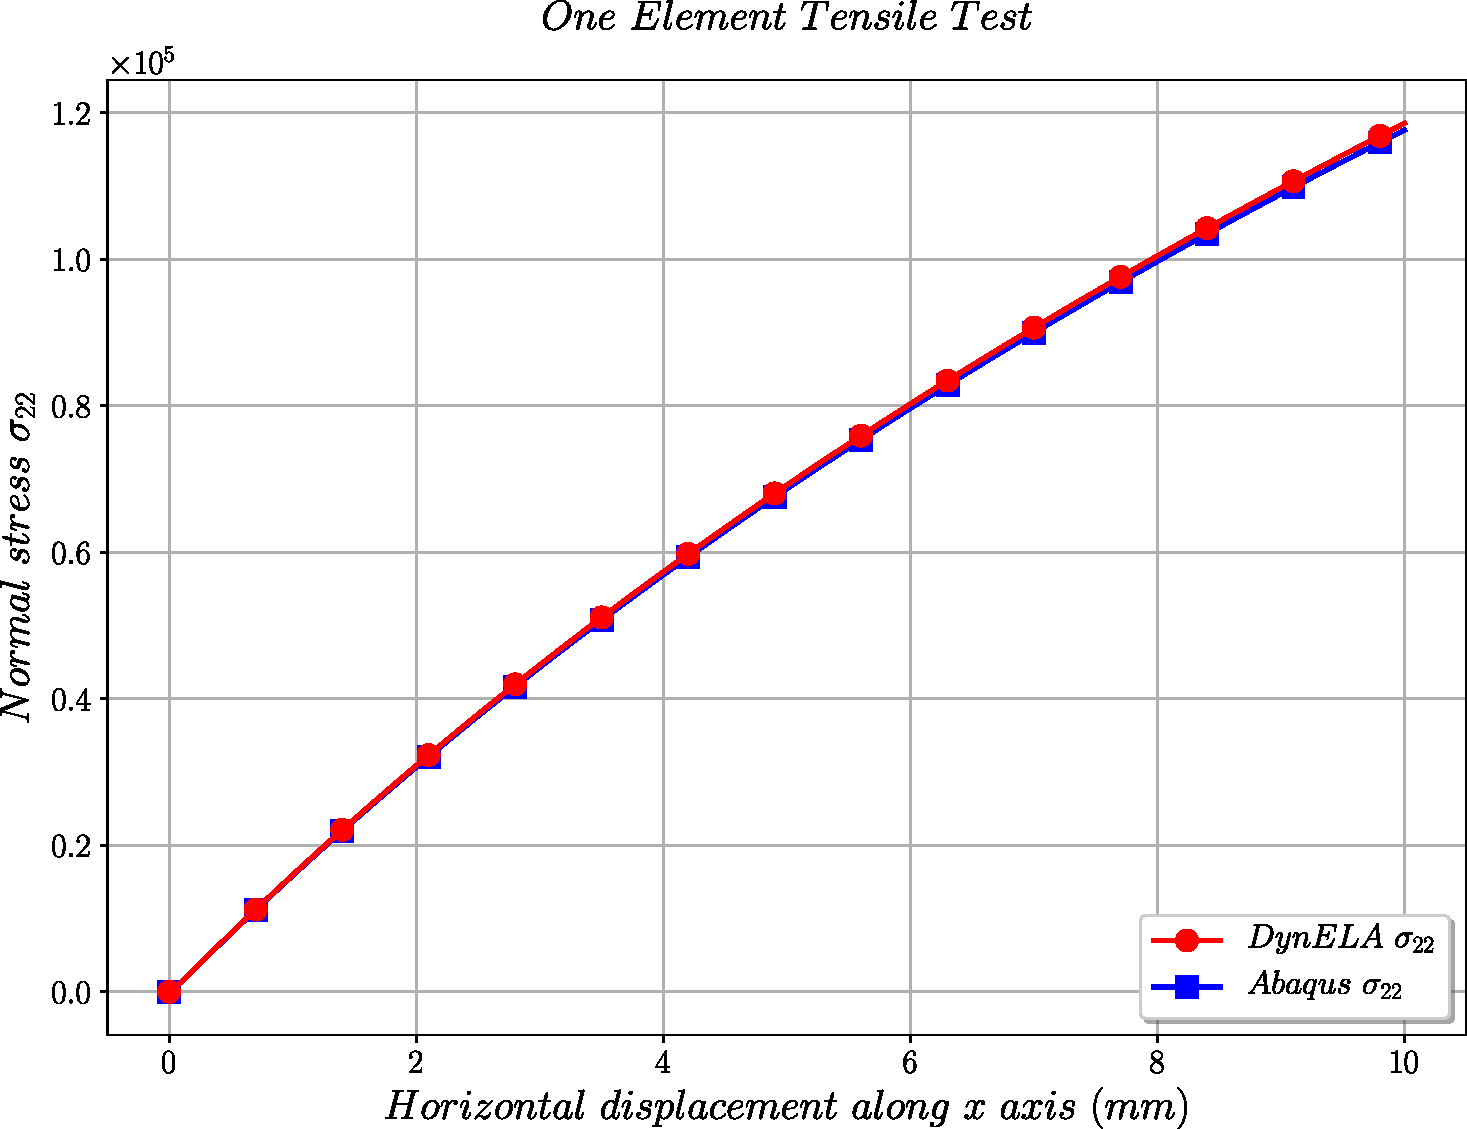
\includegraphics[width=0.45\columnwidth]{Figures/Samples/Element/Tensile_stress_22}\tabularnewline
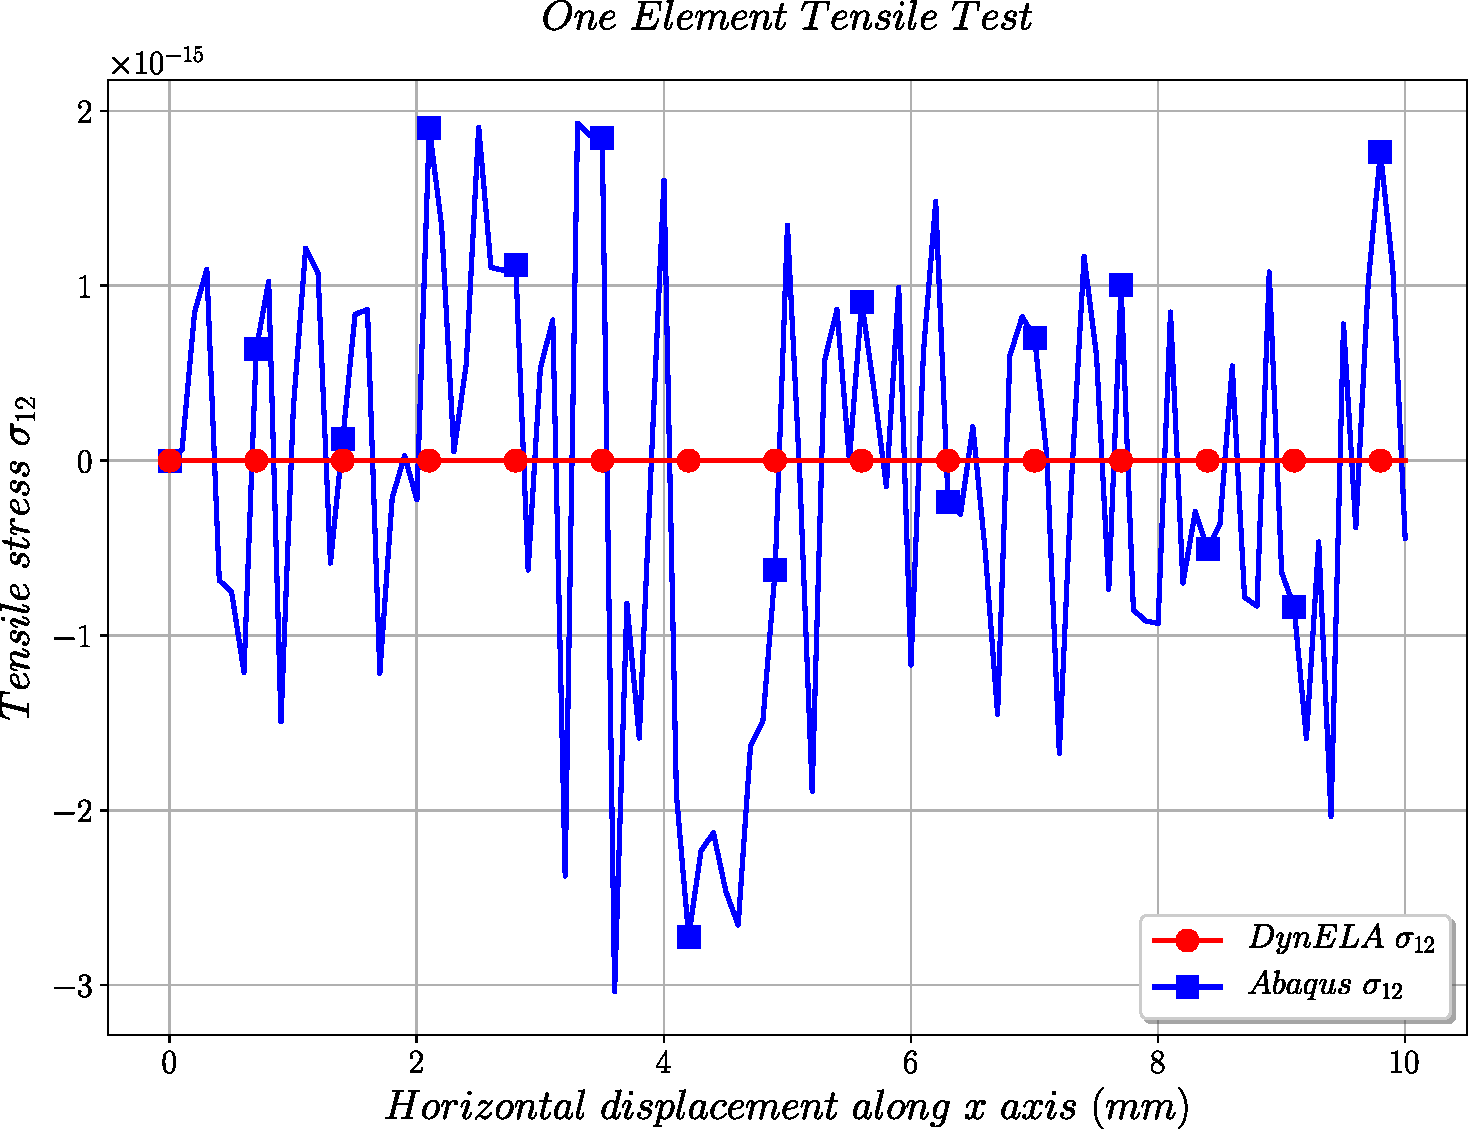
\includegraphics[width=0.45\columnwidth]{Figures/Samples/Element/Tensile_stress_12} & 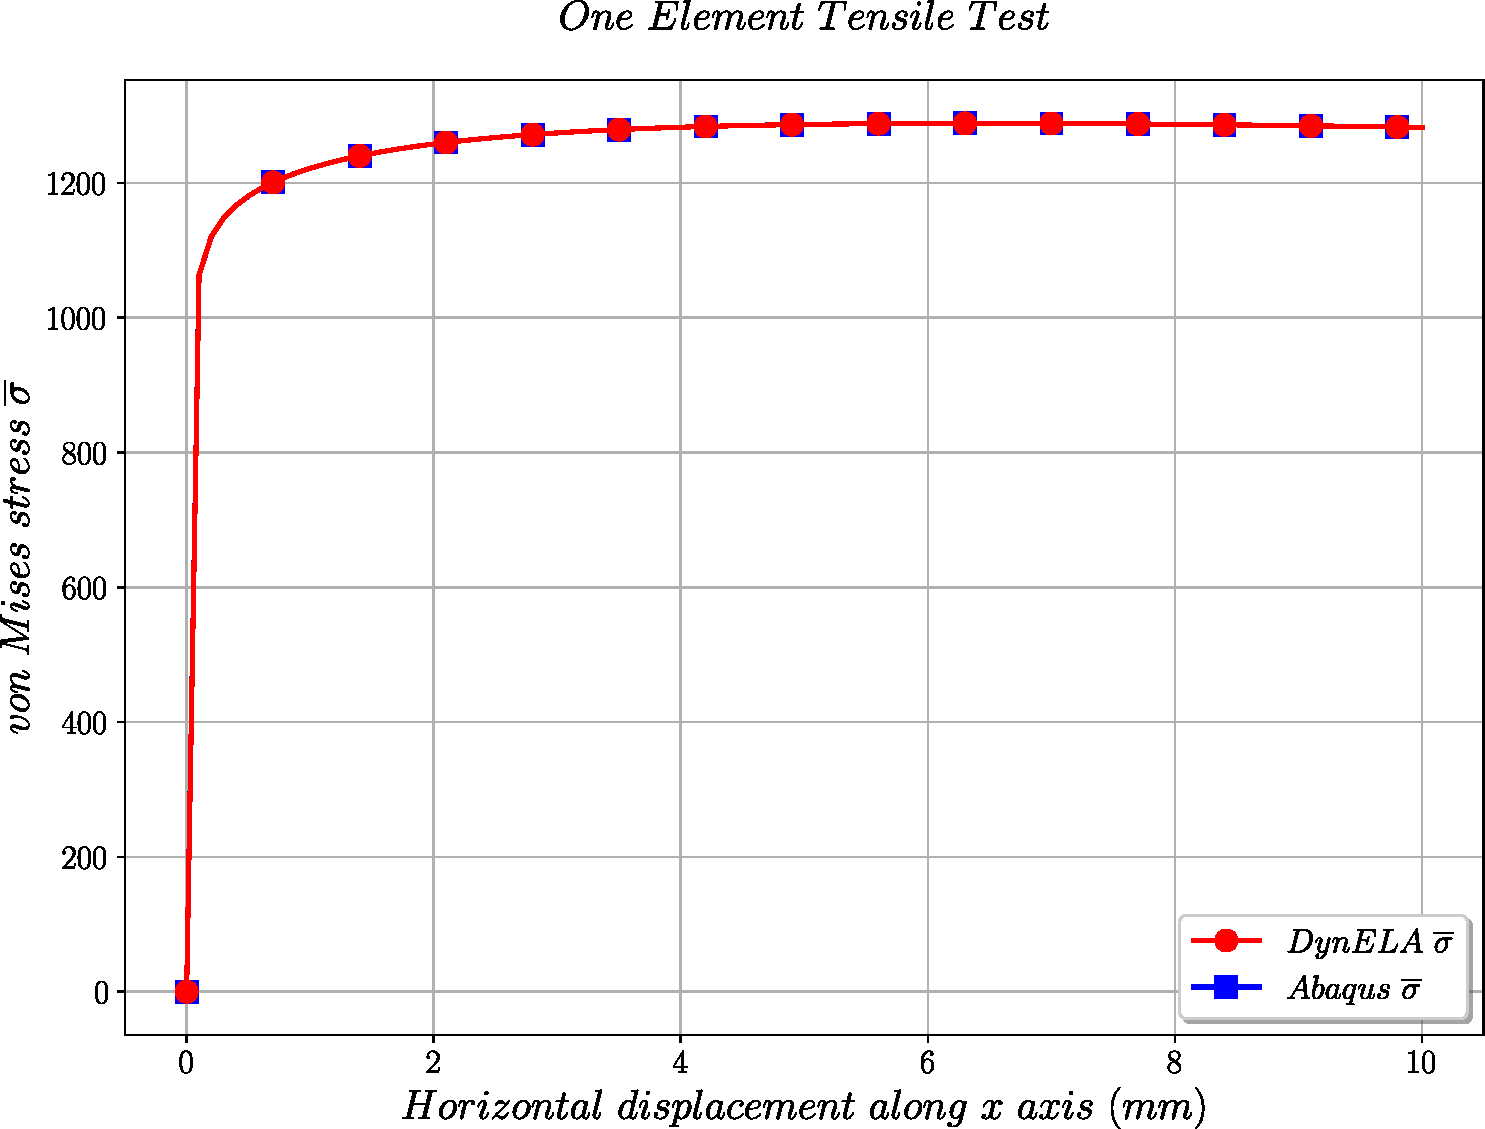
\includegraphics[width=0.45\columnwidth]{Figures/Samples/Element/Tensile_vonMises}\tabularnewline
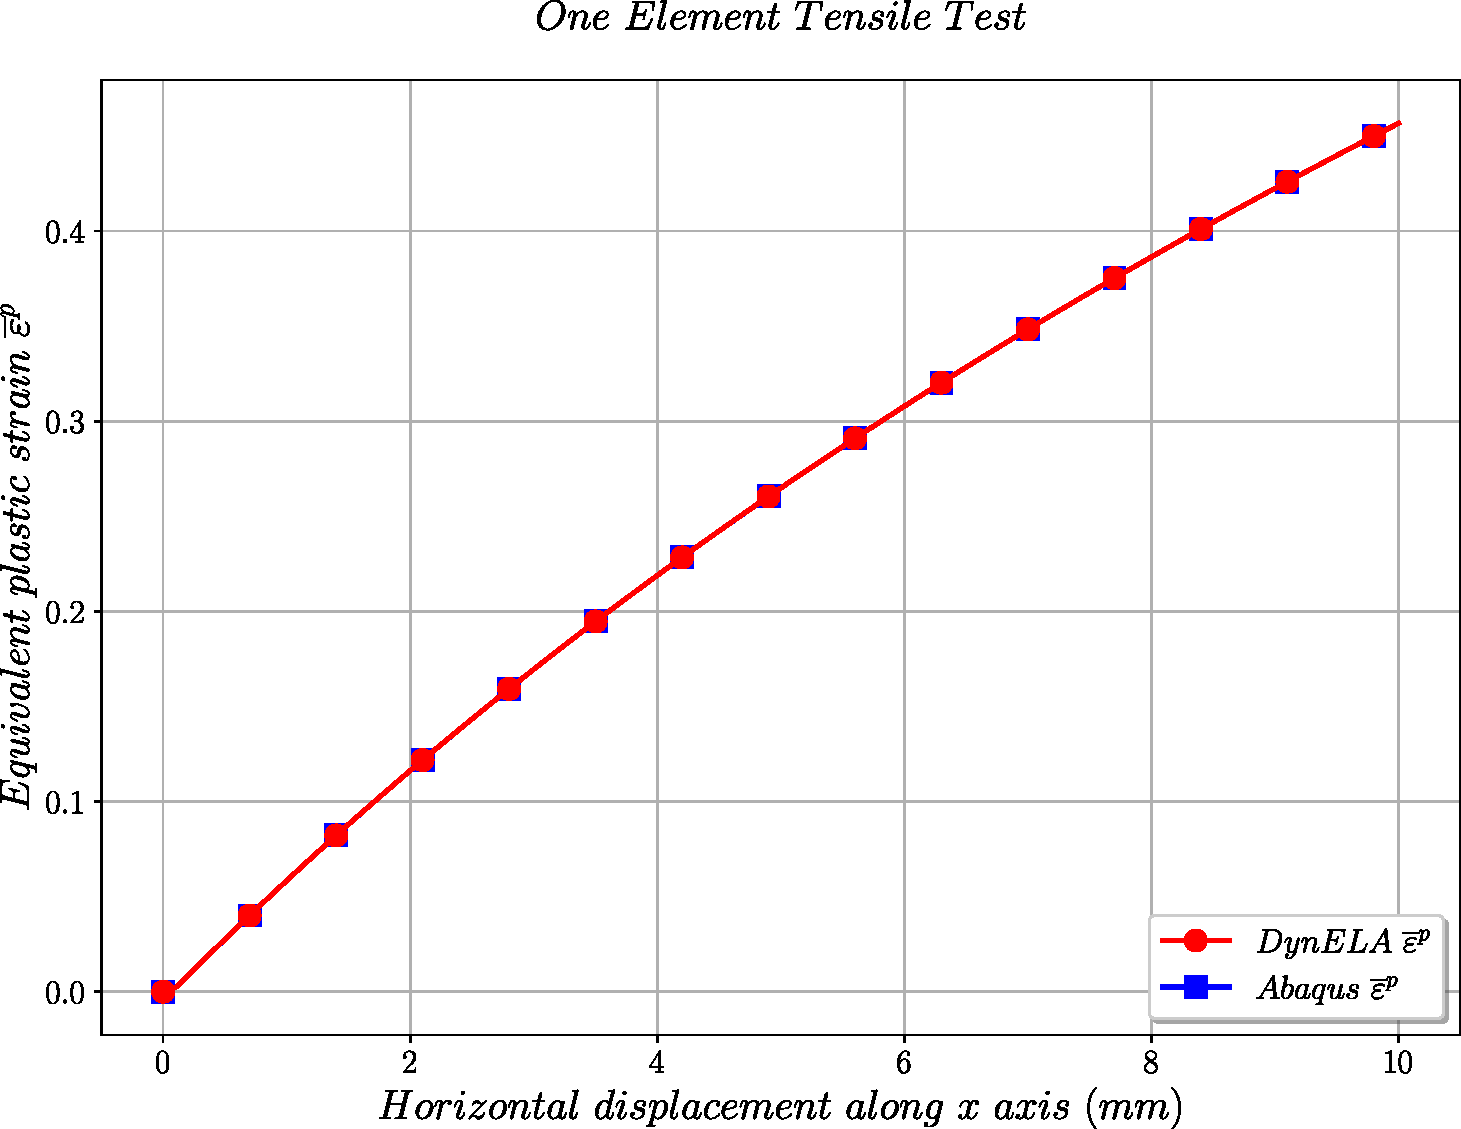
\includegraphics[width=0.45\columnwidth]{Figures/Samples/Element/Tensile_plasticStrain} & 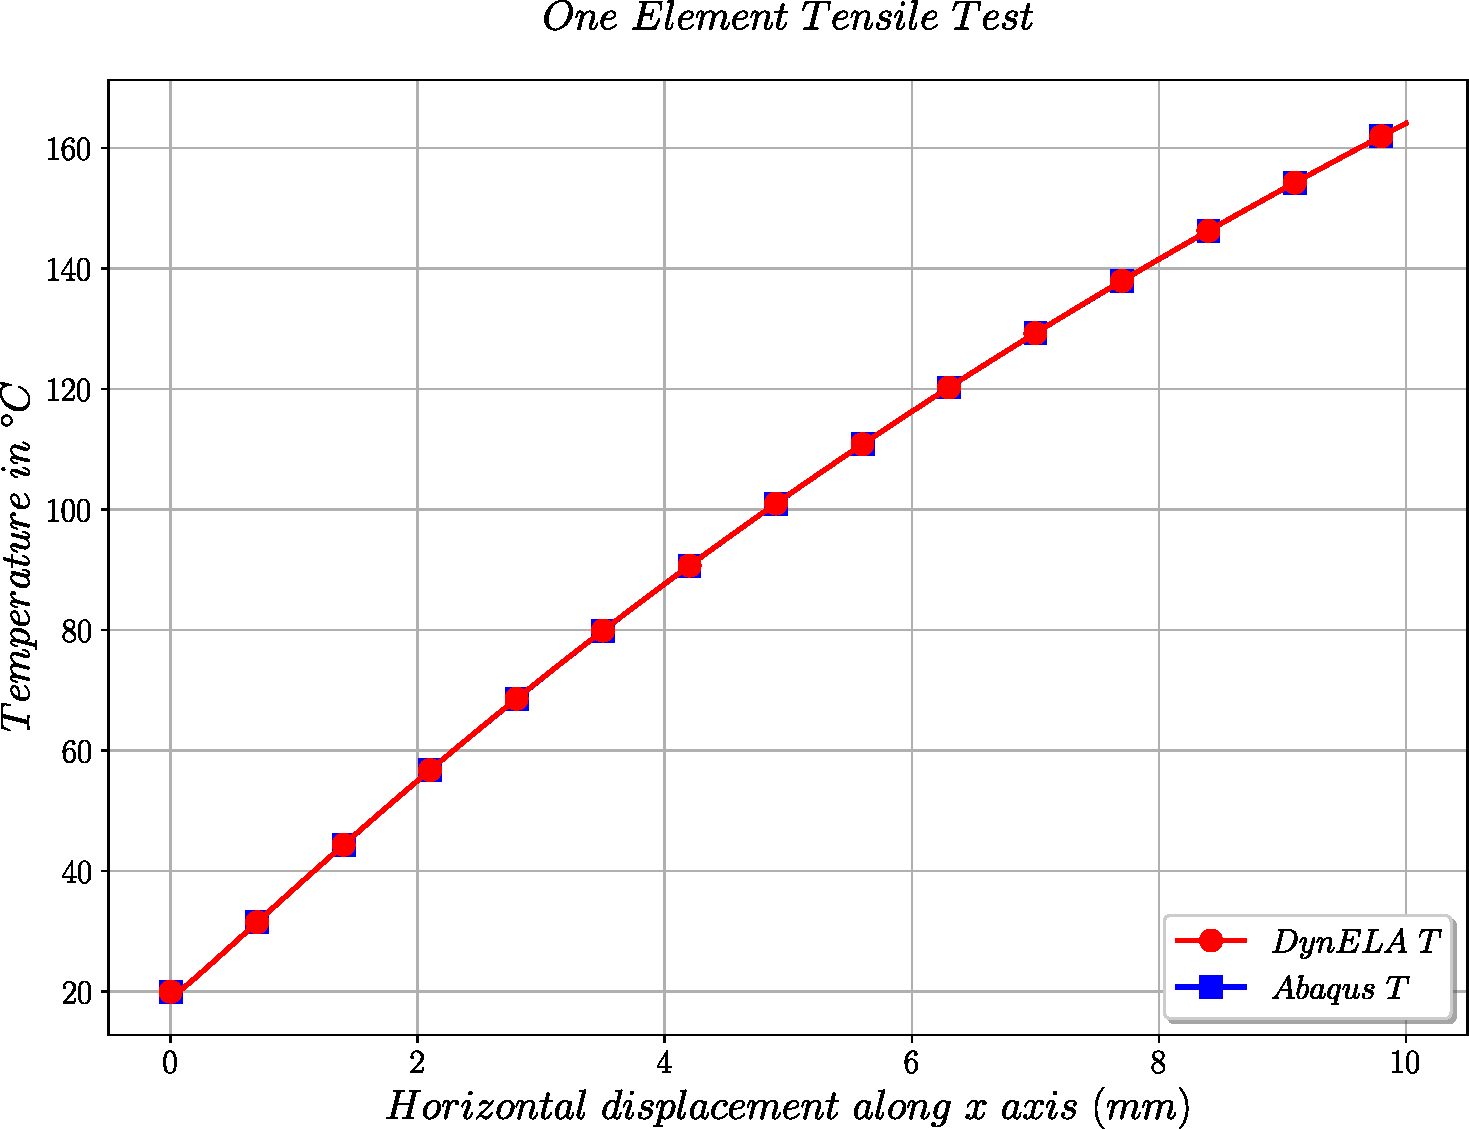
\includegraphics[width=0.45\columnwidth]{Figures/Samples/Element/Tensile_temperature}\tabularnewline
\end{tabular}
\par\end{centering}
\caption{Comparison of numerical and analytical results for the one element
tensile test\label{fig:Samples!Single!Tensile-Comparison}}
\end{figure}
\clearpage

\subsection{Element 3D tensile test}

The uniaxial one element 3D tensile test is a numerical test where
a 3D brick element (with a cubic prescribed shape) is subjected to
radial tensile as presented in figure \ref{fig:Samples!Single!Tensile-3D}.
No boundary condition has been prescribed on the $\overrightarrow{z}$
direction, so that the reduction of the width during the test can
occur. The initial shape of the specimen is $10\,mm\times10\,mm\times10\,mm$
and the the two left nodes of the element are restrained for their
displacements along the $\overrightarrow{x}$ and $\overrightarrow{y}$
directions and a prescribed horizontal displacement $d=10\,mm$ is
applied on the two right nodes of the same element as illustrated
in Figure \ref{fig:Samples!Single!Tensile-3D}. As we are using an
explicit integration scheme, the total simulation time is set to $t=0.01\,s$.
\begin{figure}[h]
\begin{centering}
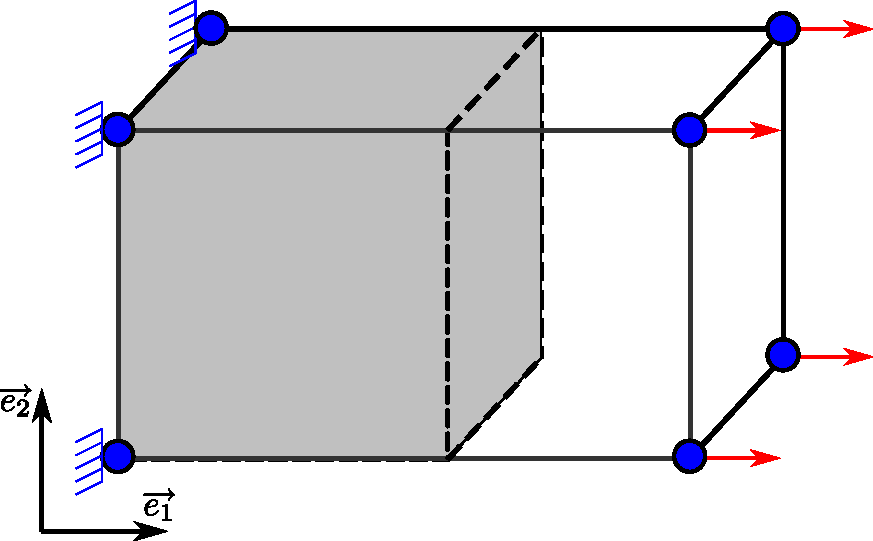
\includegraphics[width=0.5\columnwidth]{Figures/SamplesSingleTensile3D}
\par\end{centering}
\caption{Numerical model for the one element tensile test\label{fig:Samples!Single!Tensile-3D}}
\end{figure}

All the properties of the constitutive law reported in Table \ref{tab:Samples!JohnsonCookParameters}
are used and the material is assumed to follow the Johnson-Cook behavior
described by equation \ref{eq:Samples!Johnson-Cook}.

Figure \ref{fig:Samples!Single!Tensile-Comparison-3D} shows the comparison
of the DynELA solver results (plotted in red) and the Abaqus numerical
results (plotted in blue) concerning the evolution of the stress components
$\sigma_{11}$, $\sigma_{22}$, $\sigma_{12}$, $\overline{\sigma}$,
$\overline{\varepsilon}^{p}$ and $T$ \versus  the horizontal displacement
of the right edge of the specimen along the horizontal axis. For the
Abaqus model, the exact same mesh has been used. Comparison of Abaqus
and DynELA results is made by averaging the DynELA and the Abaqus
results on the $8$ integration points of the element.

\begin{figure}[h]
\begin{centering}
\begin{tabular}{cc}
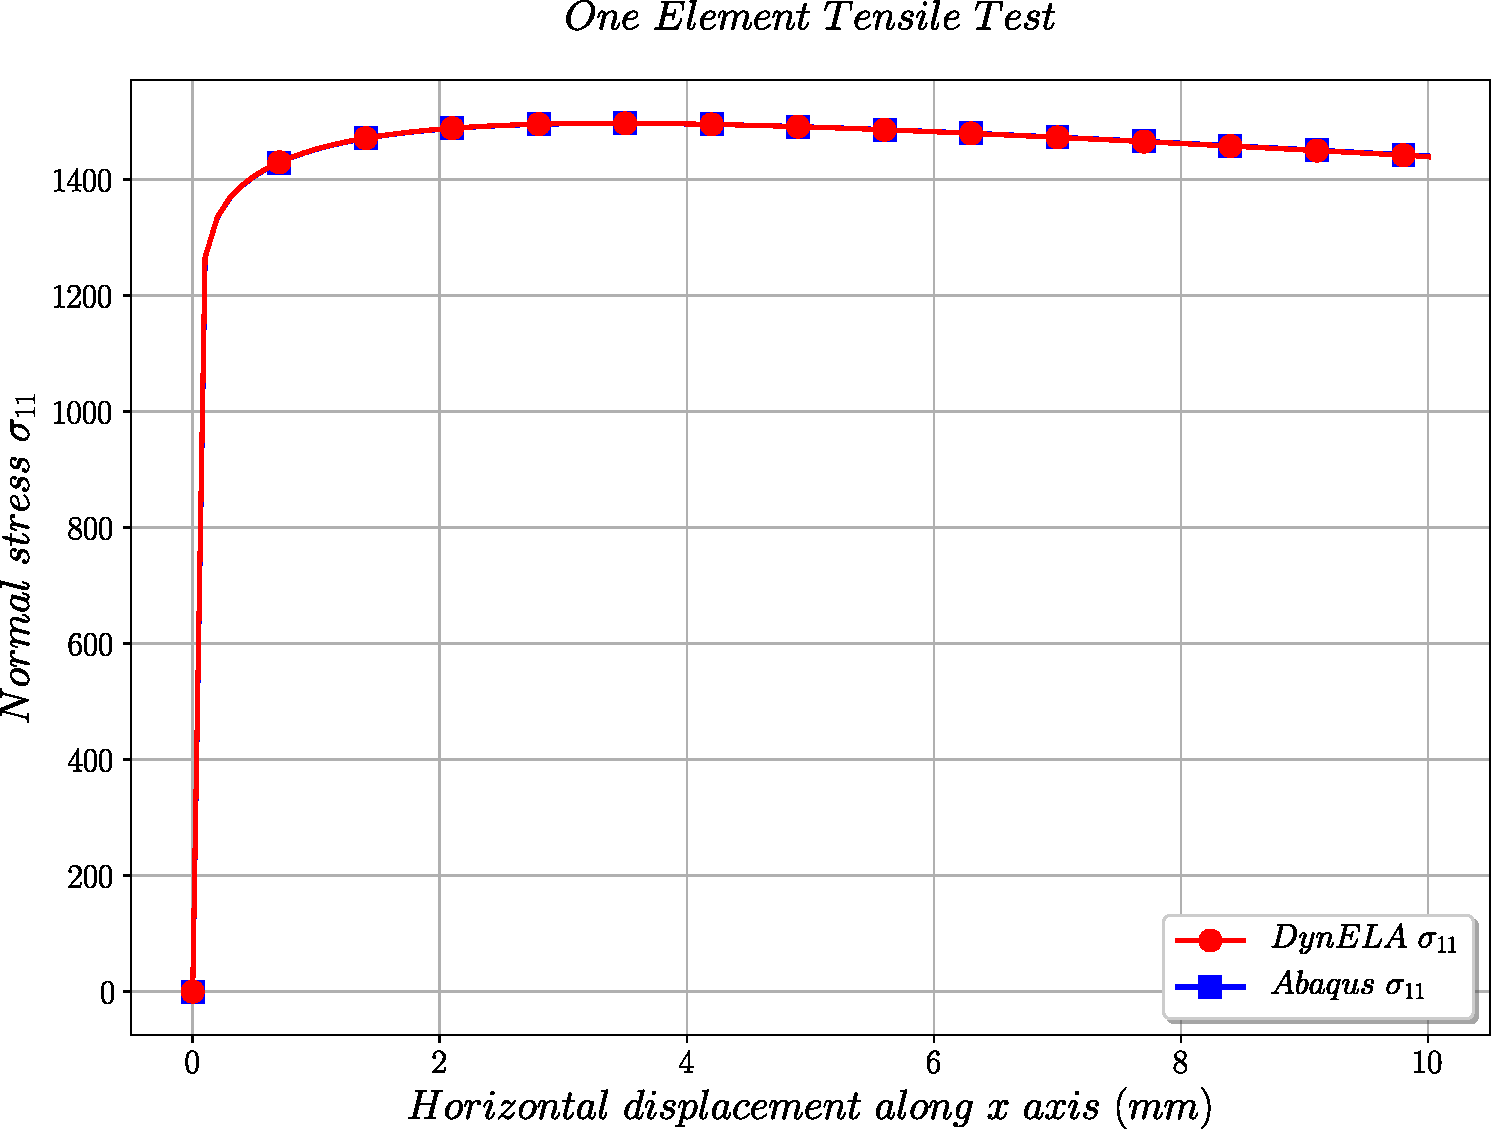
\includegraphics[width=0.45\columnwidth]{Figures/Samples/Element/Tensile3D_stress_11} & 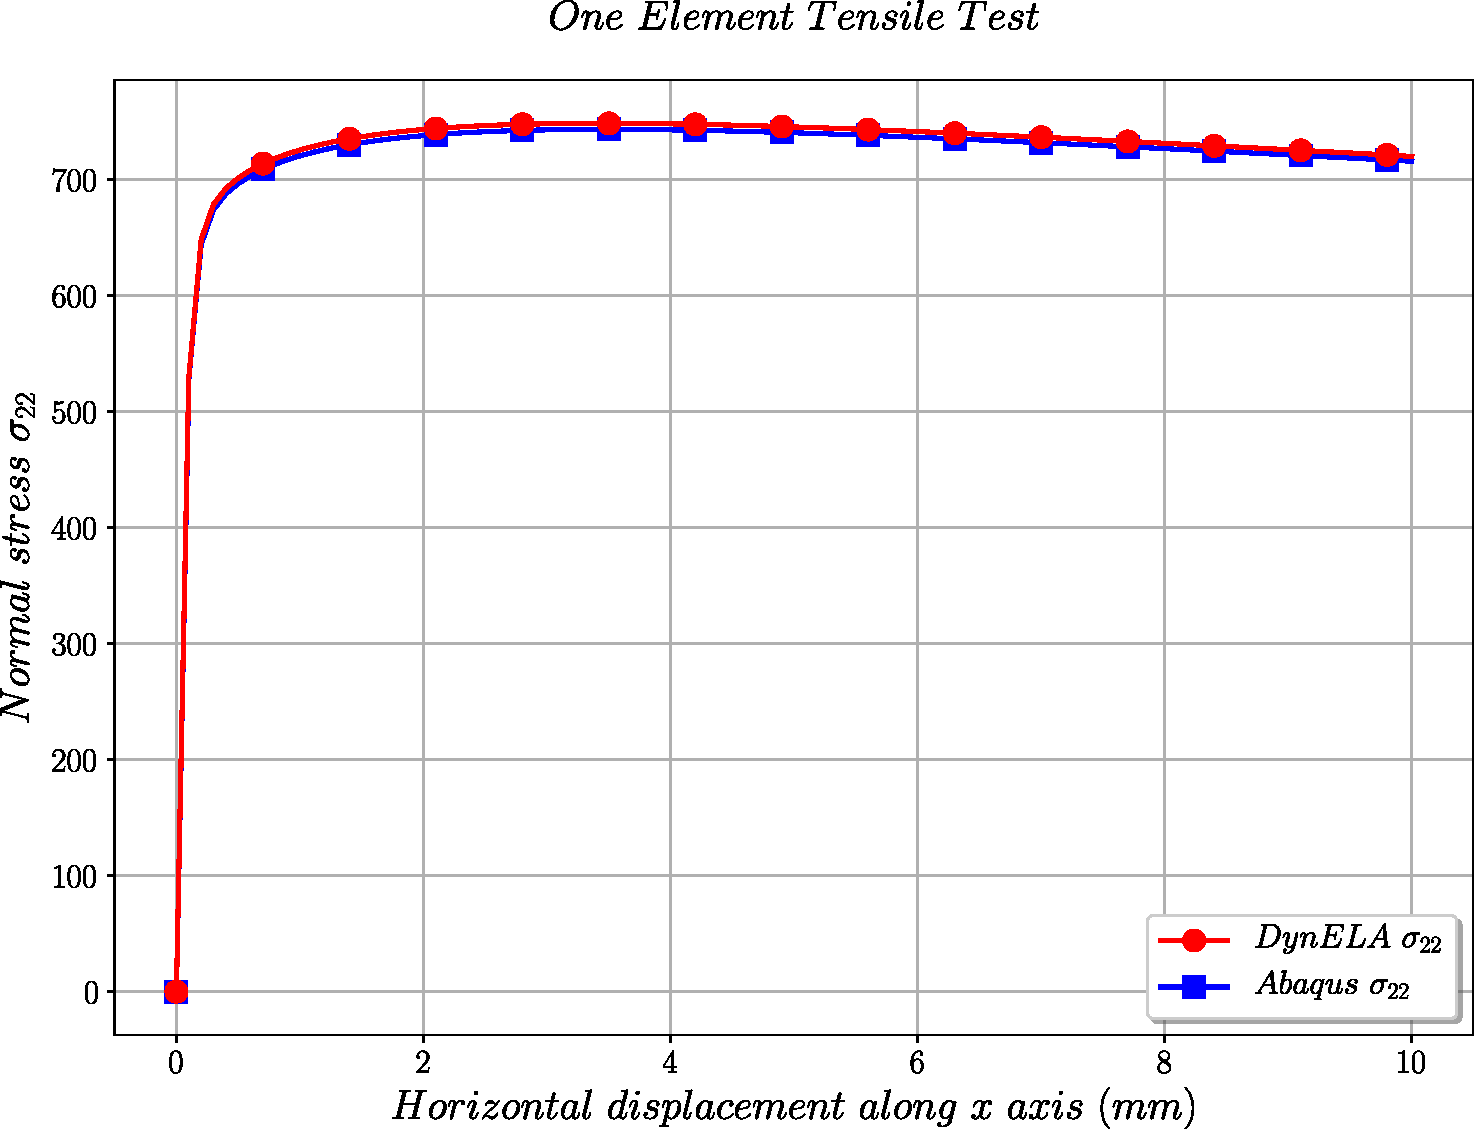
\includegraphics[width=0.45\columnwidth]{Figures/Samples/Element/Tensile3D_stress_22}\tabularnewline
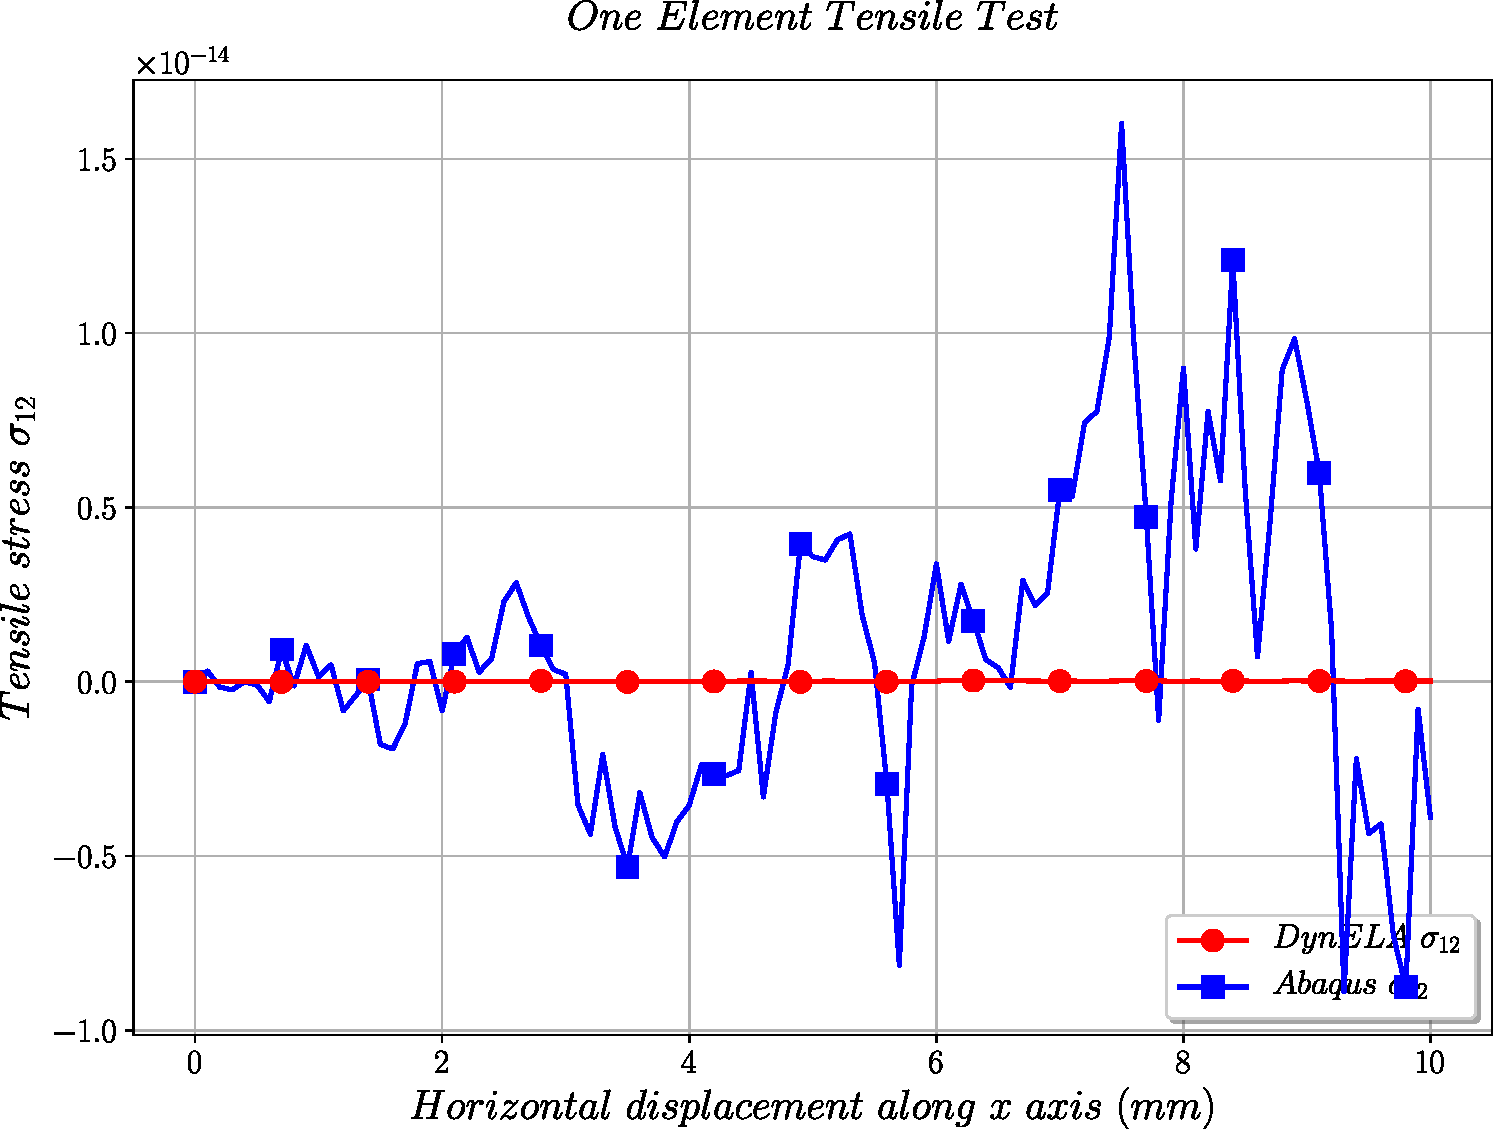
\includegraphics[width=0.45\columnwidth]{Figures/Samples/Element/Tensile3D_stress_12} & 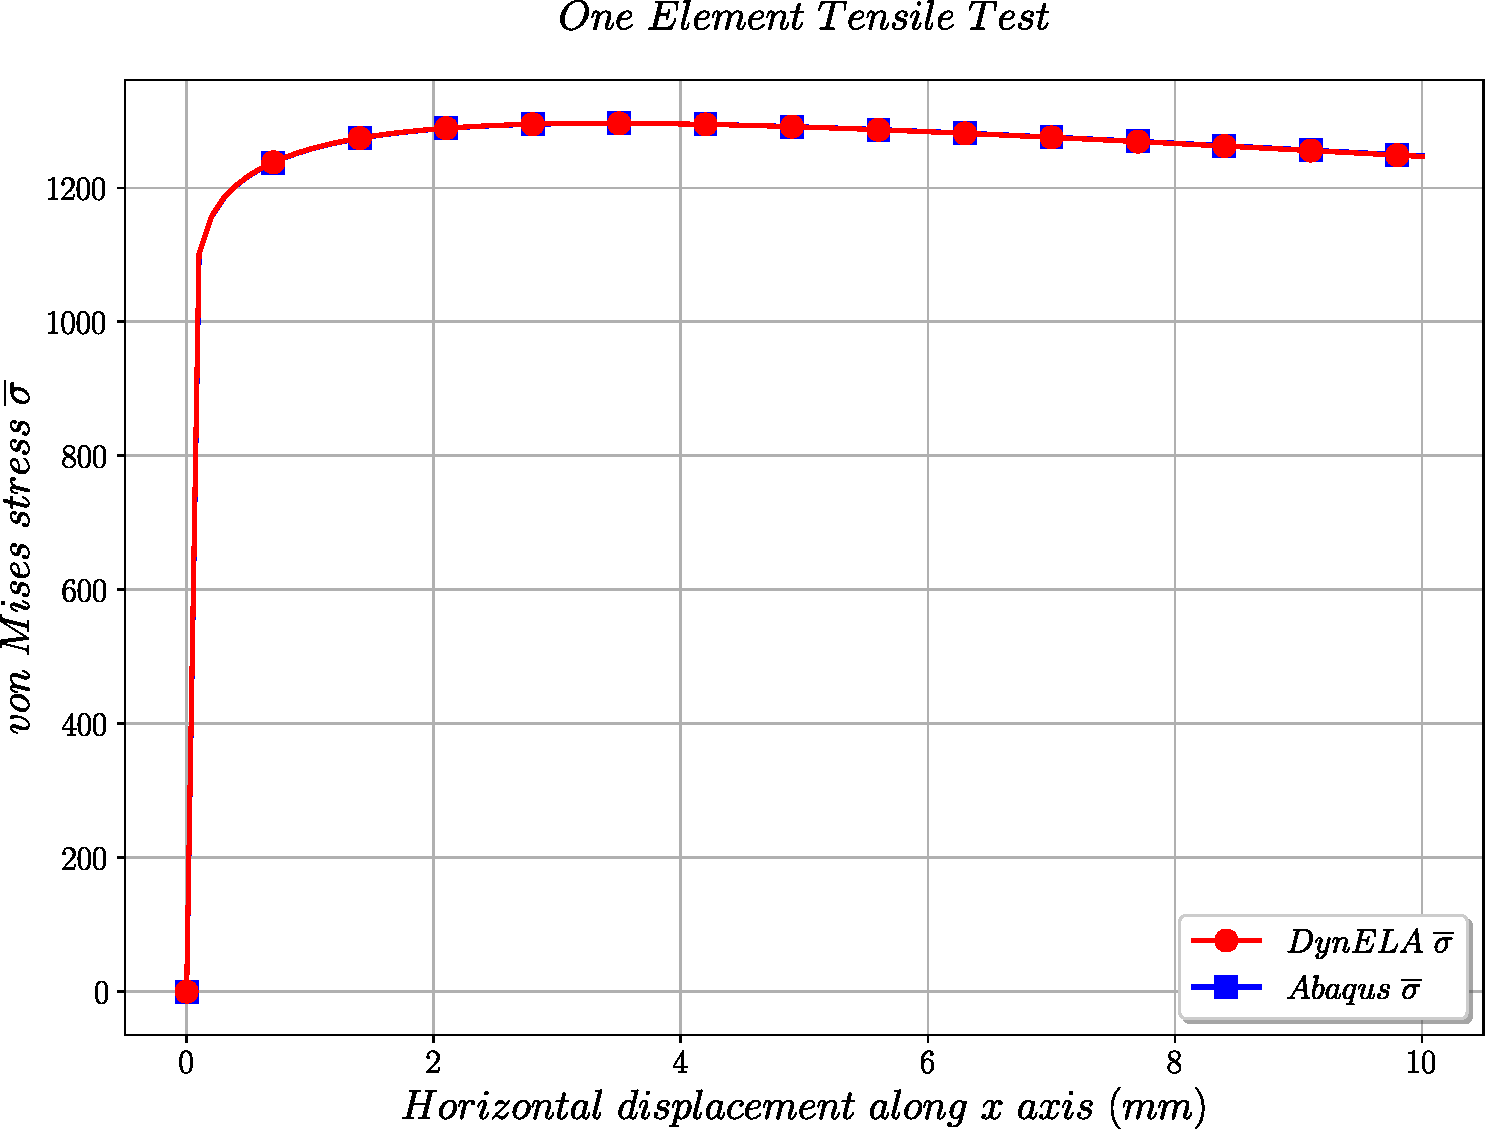
\includegraphics[width=0.45\columnwidth]{Figures/Samples/Element/Tensile3D_vonMises}\tabularnewline
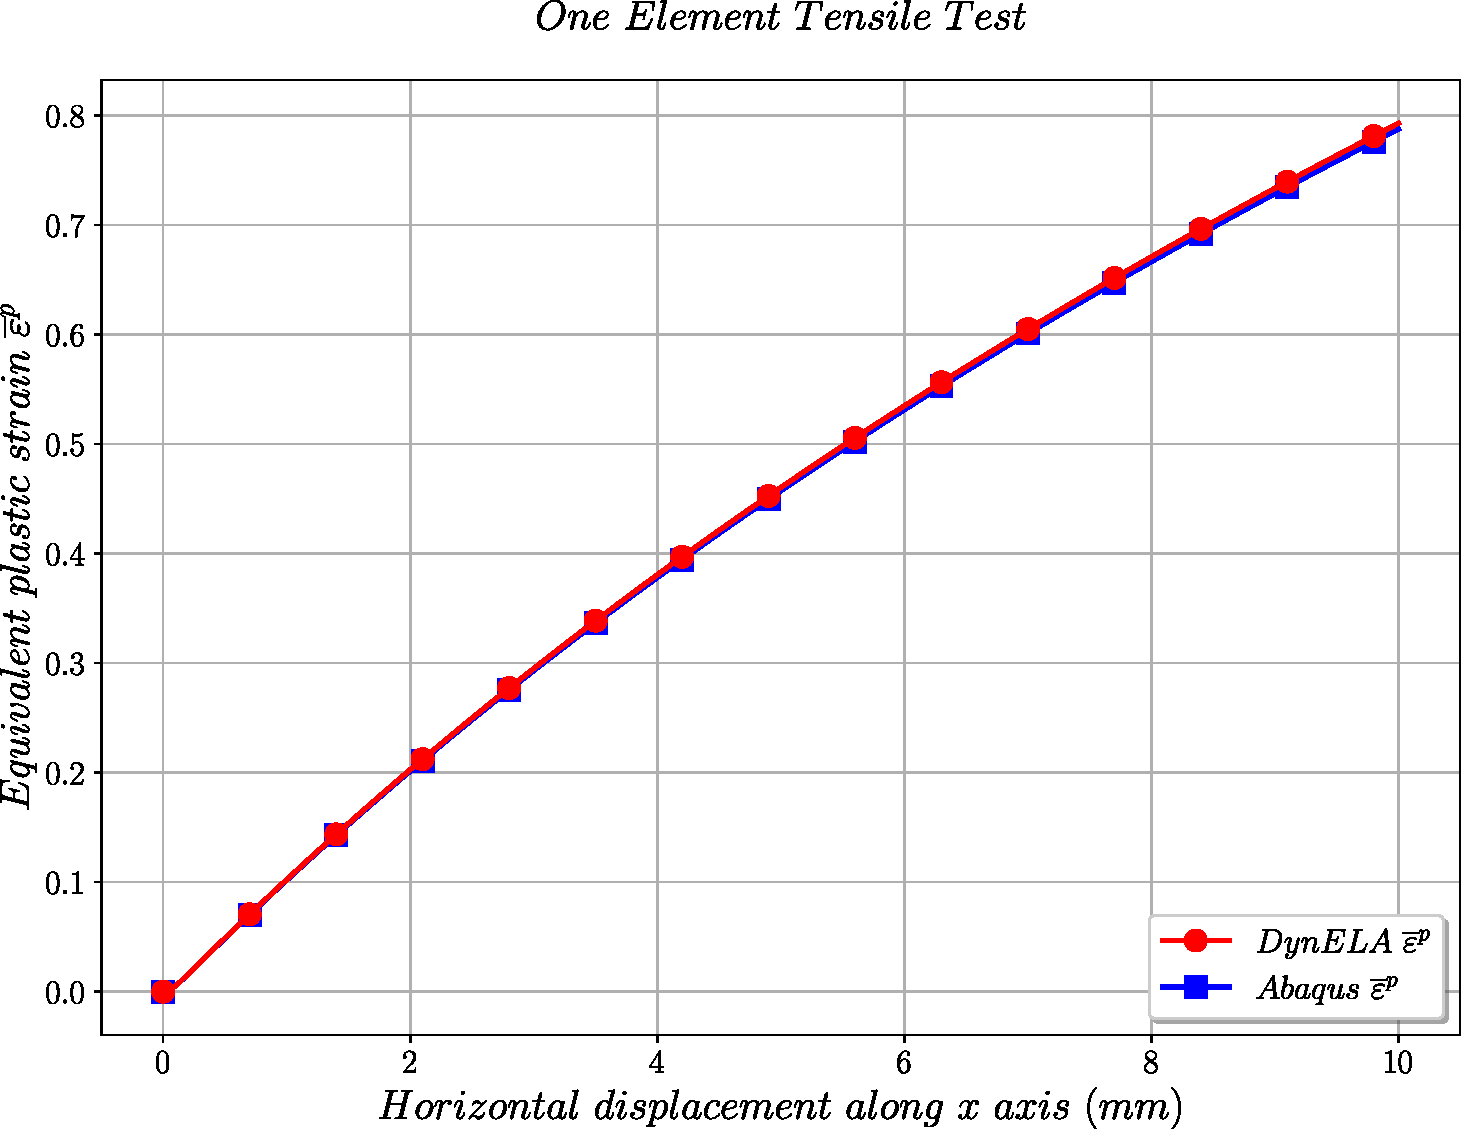
\includegraphics[width=0.45\columnwidth]{Figures/Samples/Element/Tensile3D_plasticStrain} & 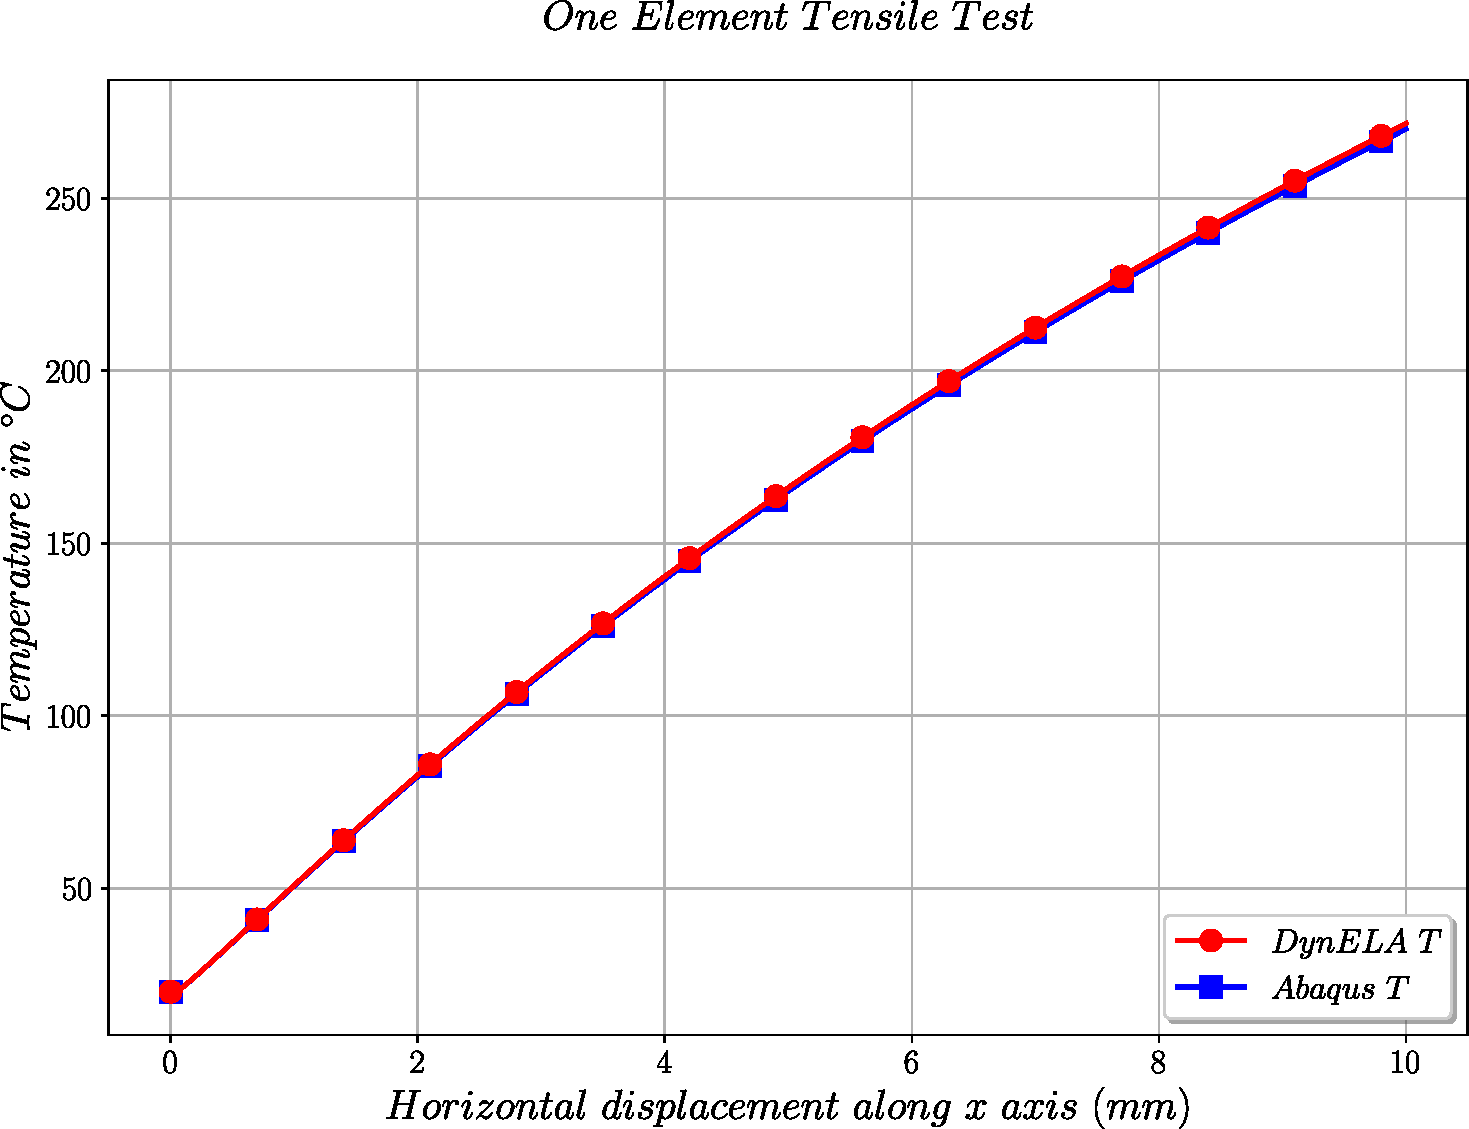
\includegraphics[width=0.45\columnwidth]{Figures/Samples/Element/Tensile3D_temperature}\tabularnewline
\end{tabular}
\par\end{centering}
\caption{Comparison of numerical and analytical results for the 3D one element
tensile test\label{fig:Samples!Single!Tensile-Comparison-3D}}
\end{figure}


\subsection{Element radial tensile test}

The uniaxial one element radial tensile test is a numerical test where
an axisymmetric element (with a square prescribed shape) is subjected
to pure radial tensile as presented in figure \ref{fig:Samples!Single!Tensile}.
The initial shape of the specimen is $10\,mm\times10\,mm$ and the
the two left nodes of the element are encastred and a prescribed horizontal
displacement $d=10\,mm$ is applied on the two right nodes of the
same element as illustrated in Figure \ref{fig:Samples!Single!Tensile}.
As we are using an explicit integration scheme, the total simulation
time is set to $t=0.01\,s$.

All the properties of the constitutive law reported in Table \ref{tab:Samples!JohnsonCookParameters}
are used and the material is assumed to follow the Johnson-Cook behavior
described by equation \ref{eq:Samples!Johnson-Cook}.

Figure \ref{fig:Samples!Single!Radial-Comparison} shows the comparison
of the DynELA solver results (plotted in red) and the Abaqus numerical
results (plotted in blue) concerning the evolution of the stress components
$\sigma_{11}$, $\sigma_{22}$, $\sigma_{12}$, $\overline{\sigma}$,
$\overline{\varepsilon}^{p}$ and $T$ \versus  the horizontal displacement
of the right edge of the specimen along the horizontal axis. Again,
comparison of Abaqus and DynELA results is made by averaging the DynELA
results on the $4$ integration points of the element because \DynELA~uses
full integrated elements while Abaqus have reduced integrated elements
only but in fact, the DynELA results at the $4$ integration points
are the same in this benchmark test.

\begin{figure}[h]
\begin{centering}
\begin{tabular}{cc}
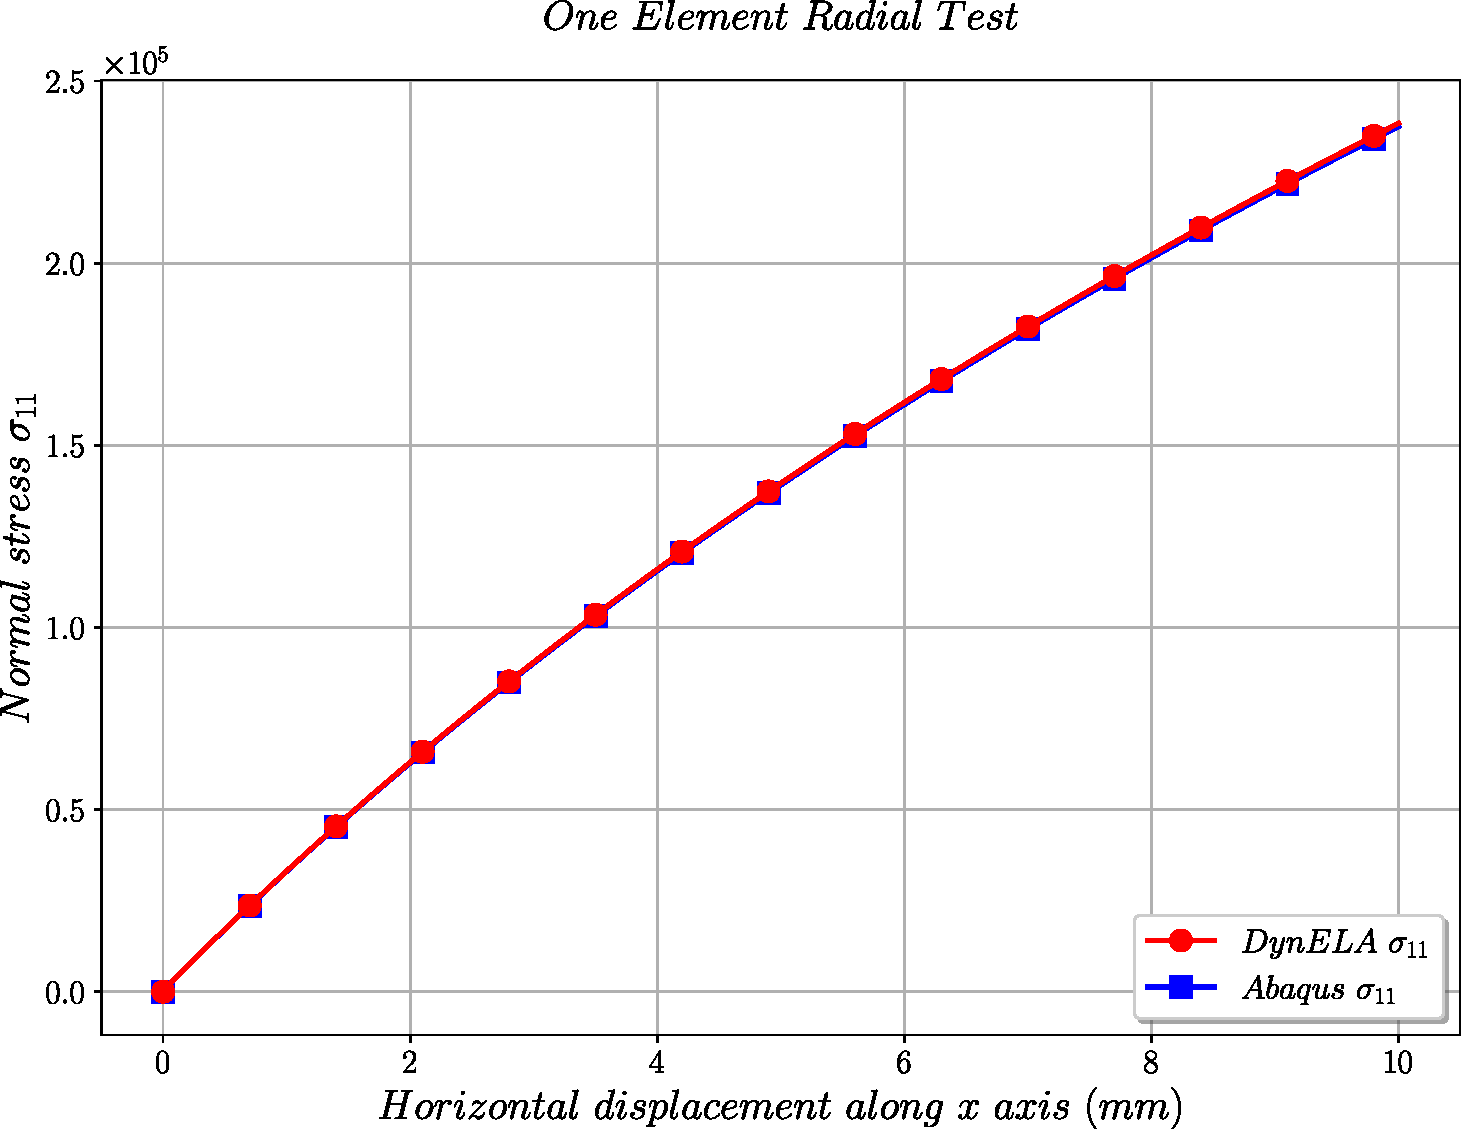
\includegraphics[width=0.45\columnwidth]{Figures/Samples/Element/Radial_stress_11} & 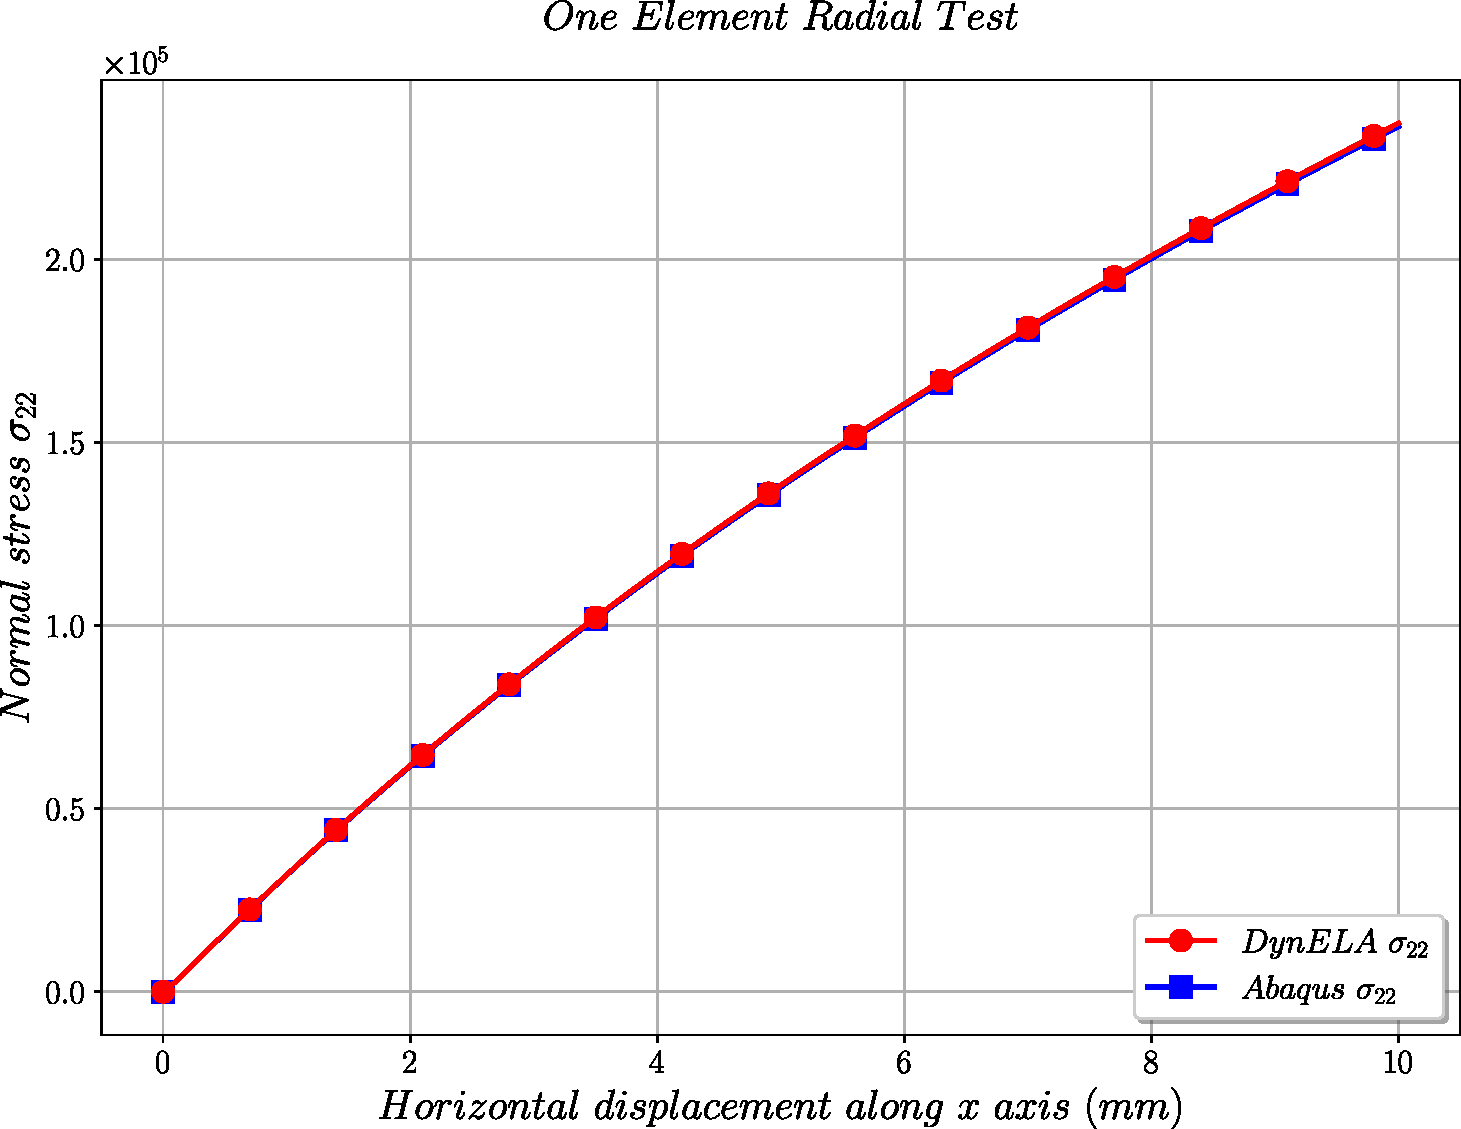
\includegraphics[width=0.45\columnwidth]{Figures/Samples/Element/Radial_stress_22}\tabularnewline
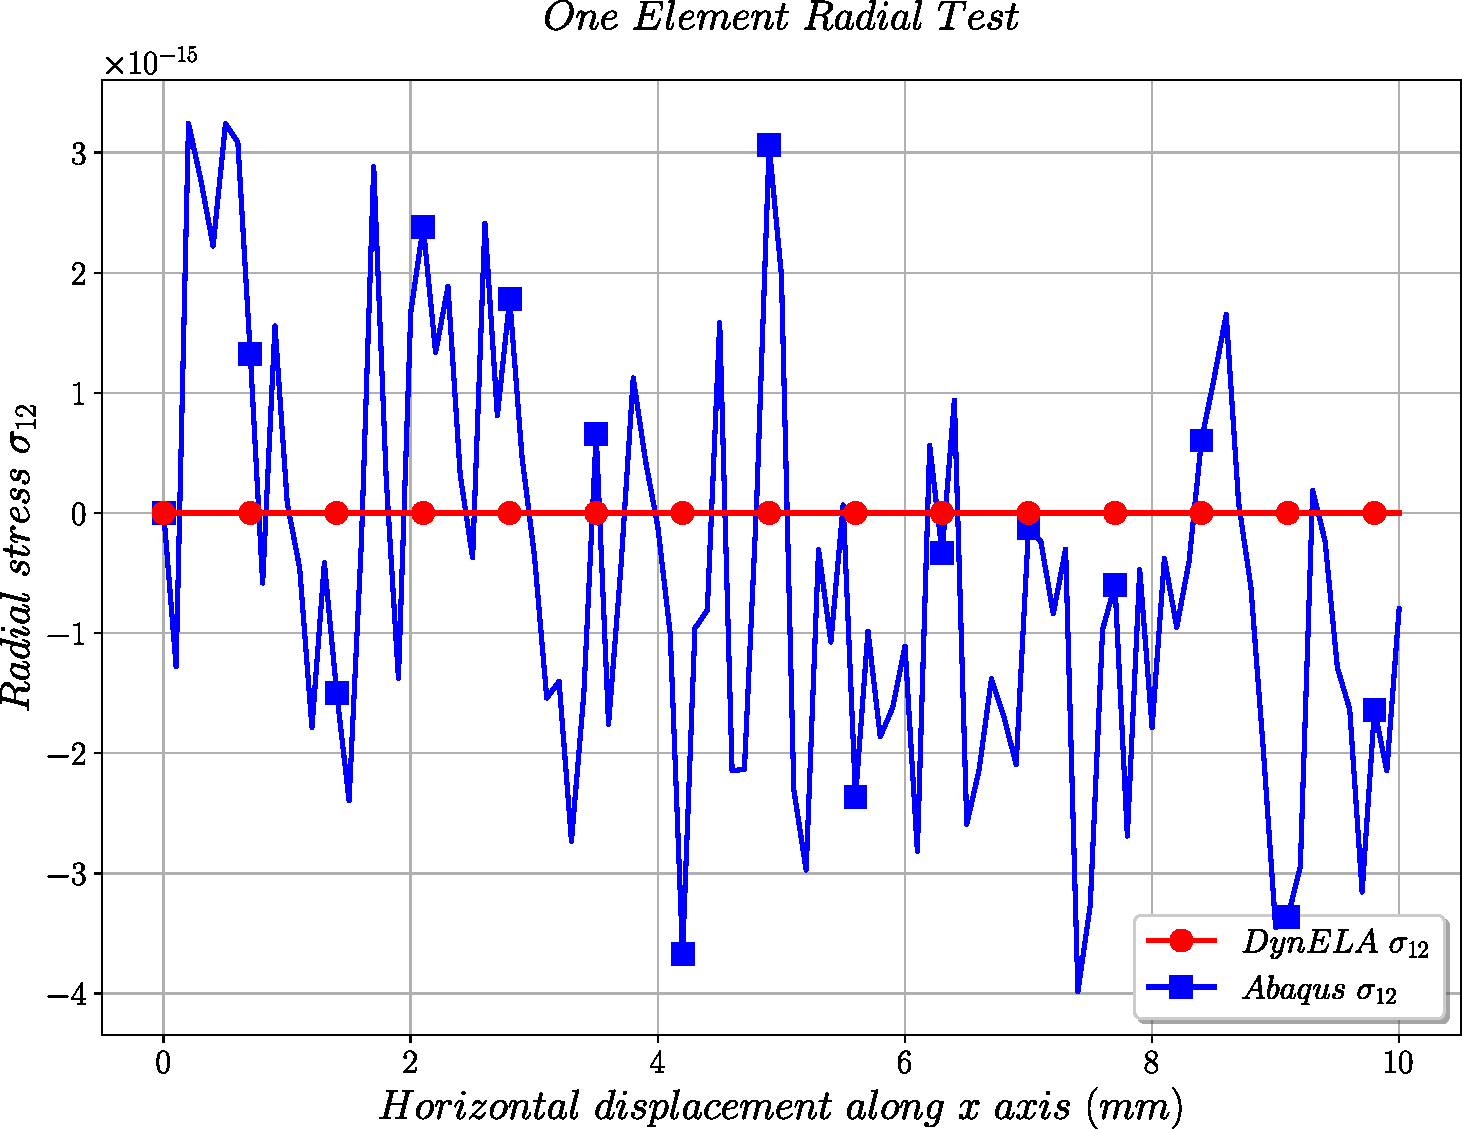
\includegraphics[width=0.45\columnwidth]{Figures/Samples/Element/Radial_stress_12} & 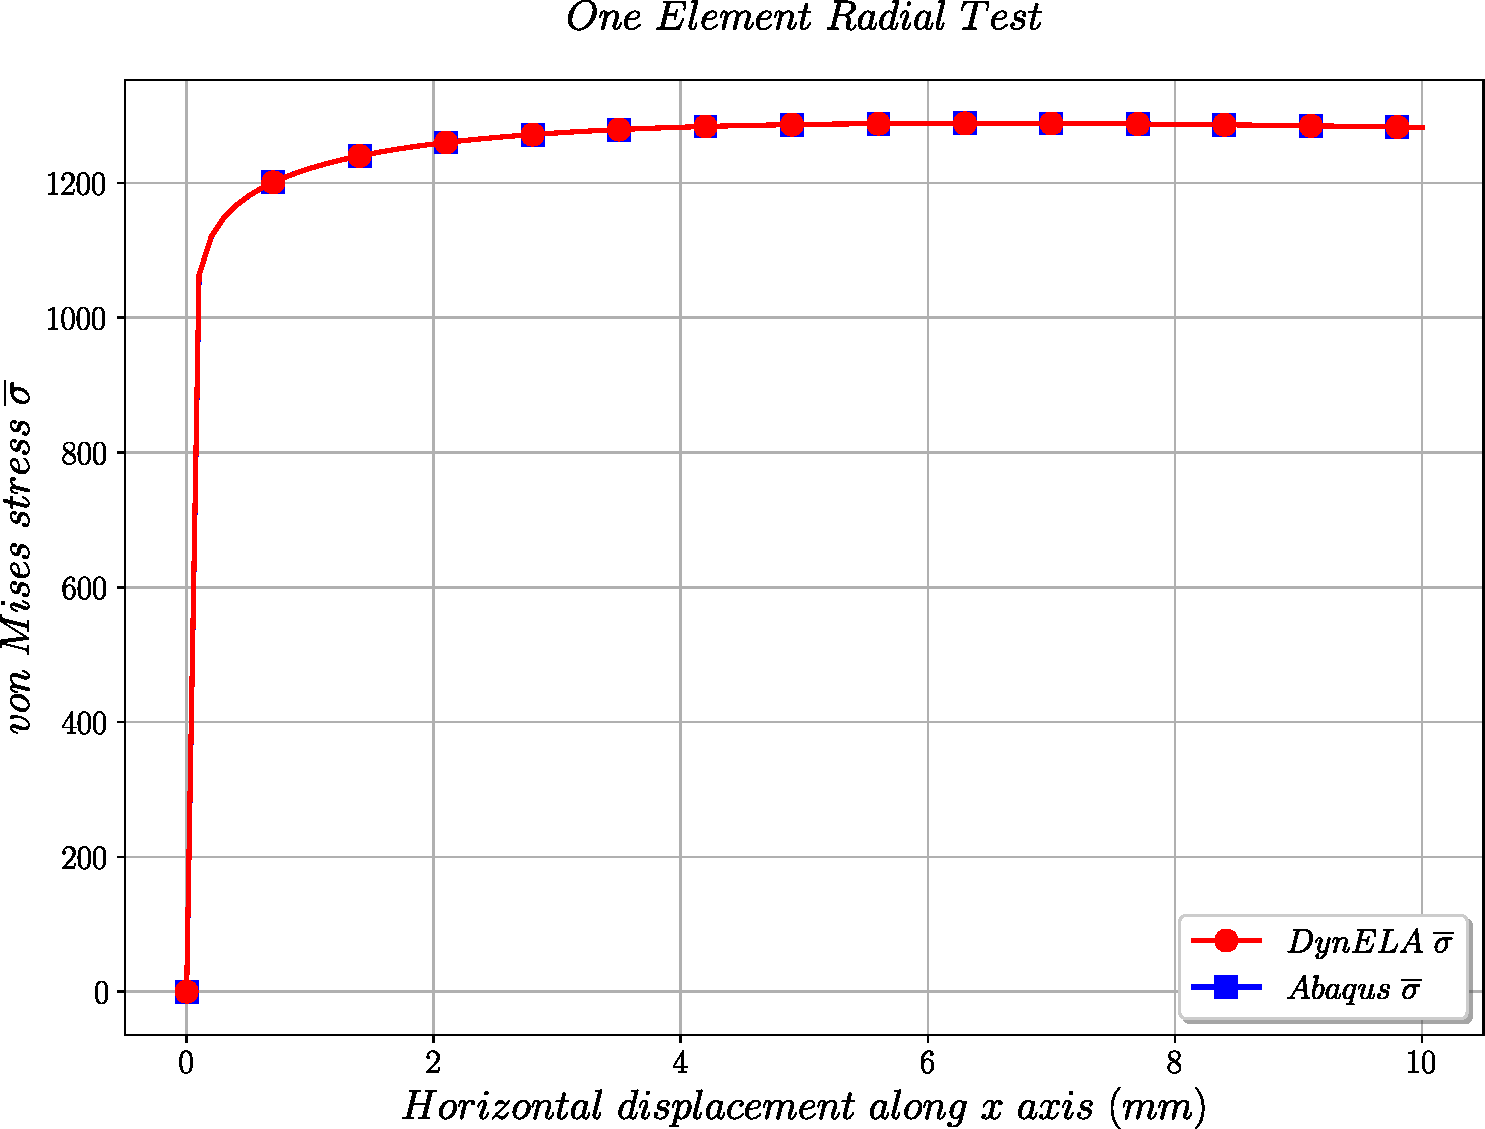
\includegraphics[width=0.45\columnwidth]{Figures/Samples/Element/Radial_vonMises}\tabularnewline
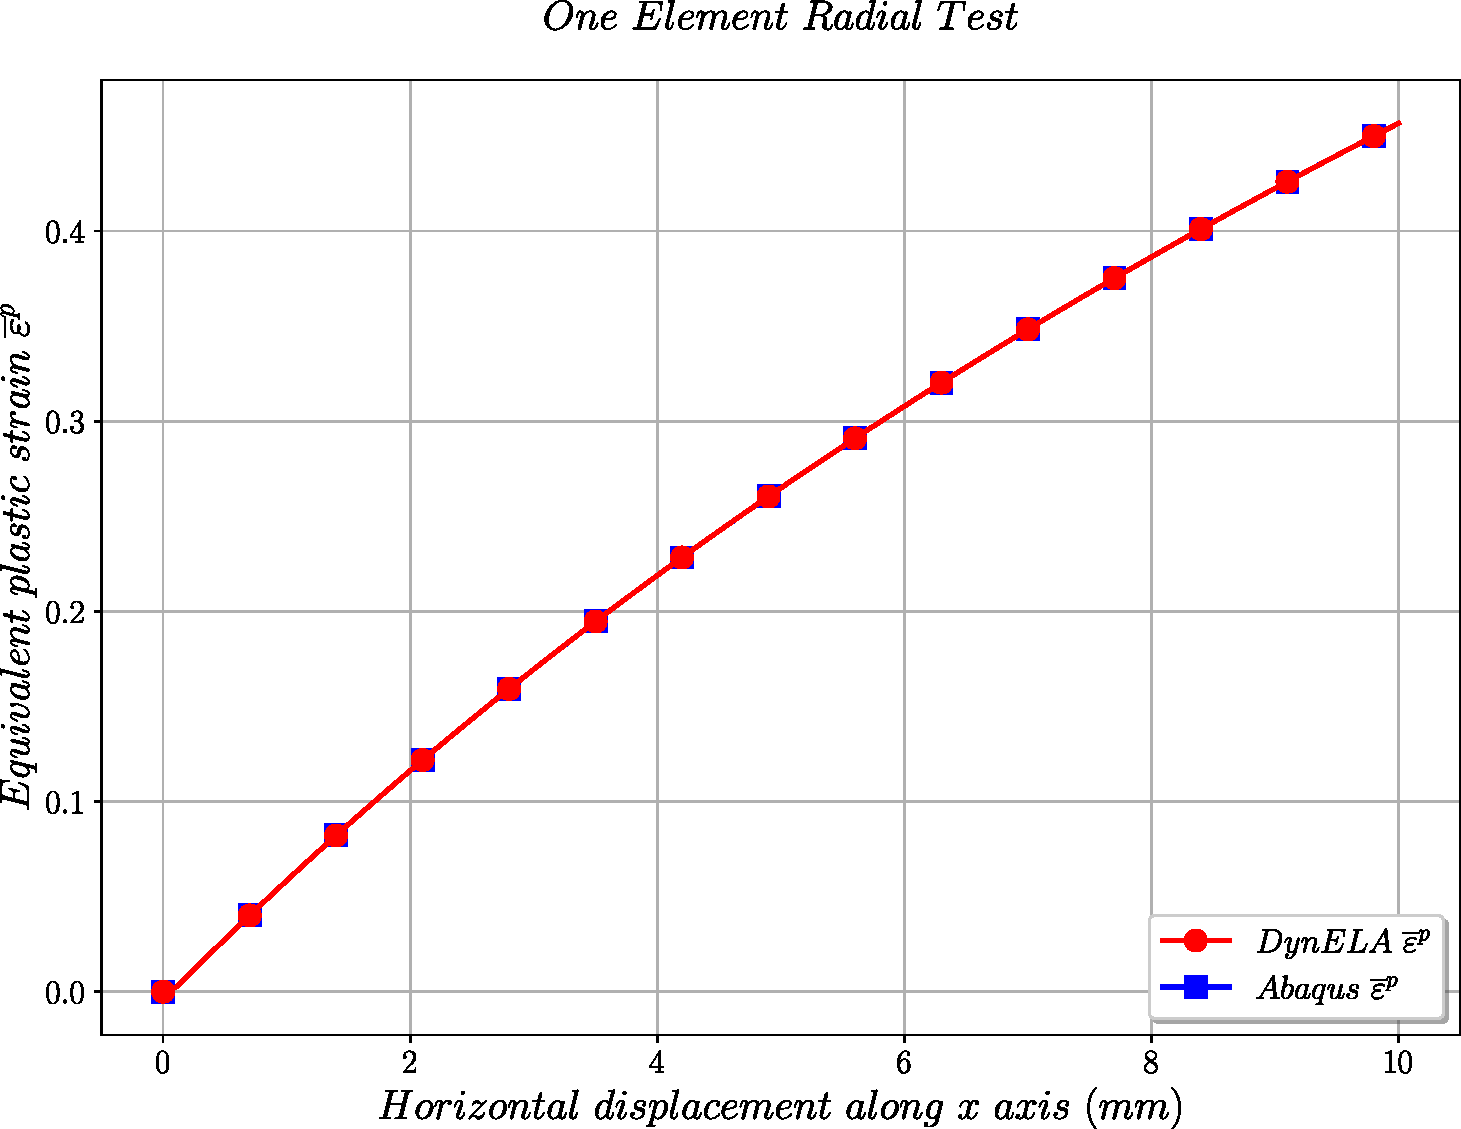
\includegraphics[width=0.45\columnwidth]{Figures/Samples/Element/Radial_plasticStrain} & 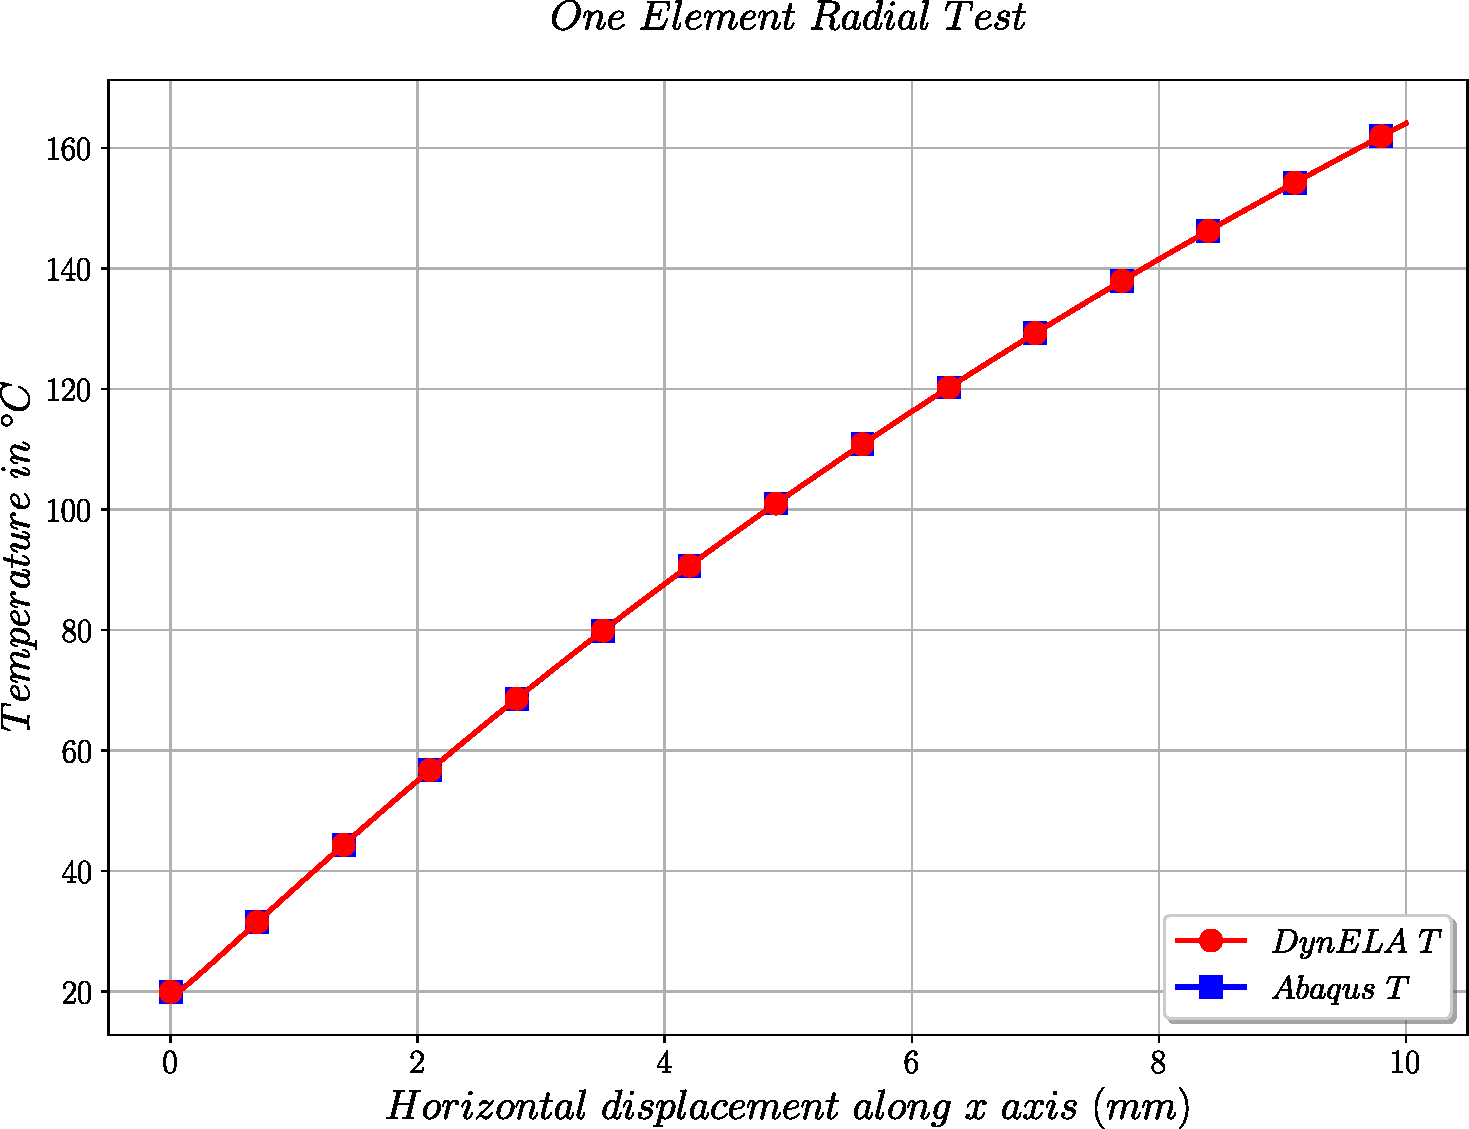
\includegraphics[width=0.45\columnwidth]{Figures/Samples/Element/Radial_temperature}\tabularnewline
\end{tabular}
\par\end{centering}
\caption{Comparison of numerical and analytical results for the one element
radial tensile test\label{fig:Samples!Single!Radial-Comparison}}
\end{figure}
\clearpage

\subsection{Element radial torus test}

The uniaxial one element torus tensile test is a numerical test where
an axisymmetric element (with a square prescribed shape) is subjected
to radial tensile as presented in figure \ref{fig:Samples!Single!Torus}.
\begin{figure}[h]
\begin{centering}
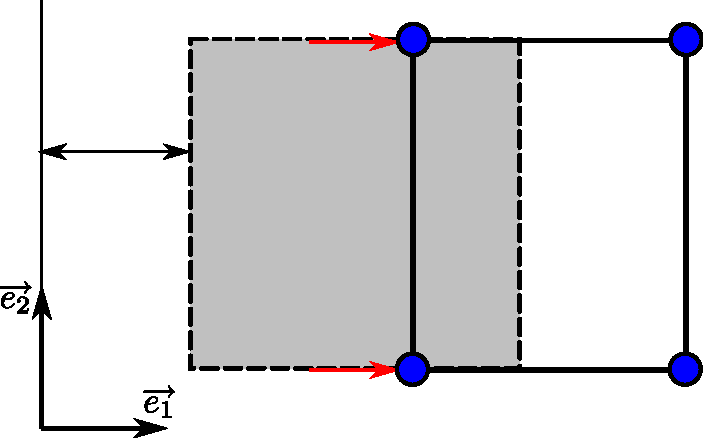
\includegraphics[width=0.5\columnwidth]{Figures/SamplesSingleTorus}
\par\end{centering}
\caption{Numerical model for the one element torus test\label{fig:Samples!Single!Torus}}
\end{figure}
 The difference with the previous test is that the left edge of the
specimen in not aligned with the symmetry axis, the radial coordinate
of the left edge is $r=10\,mm$. The initial shape of the specimen
is $10\,mm\times10\,mm$ and a prescribed horizontal displacement
$d=10\,mm$ is applied on the two left nodes of the element as illustrated
in Figure \ref{fig:Samples!Single!Torus}. As we are using an explicit
integration scheme, the total simulation time is set to $t=0.01\,s$.
All the properties of the constitutive law reported in Table \ref{tab:Samples!JohnsonCookParameters}
are used and the material is assumed to follow the Johnson-Cook behavior
described by equation \ref{eq:Samples!Johnson-Cook}.

As a global comparison, Figure \ref{fig:Samples!Single!Torus-Comparison-ux}
show the comparison of the right edge displacement \versus the left
edge displacement for both the DynELA and the Abaqus simulations.
\begin{figure}[h]
\begin{centering}
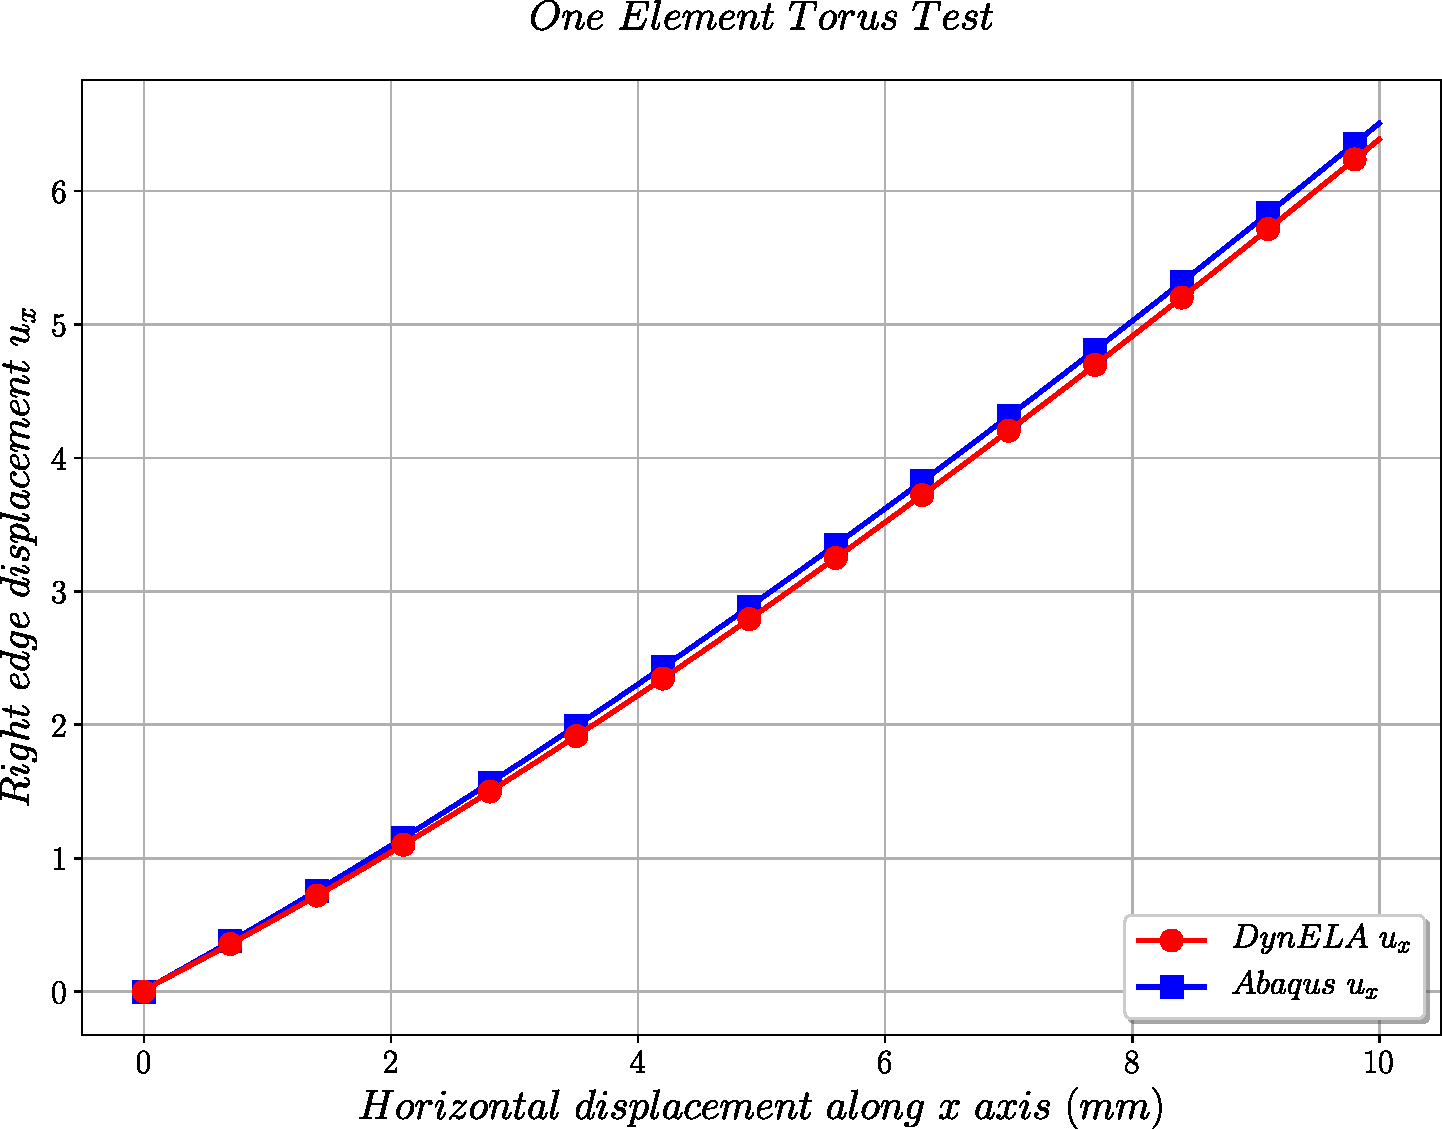
\includegraphics[width=0.5\columnwidth]{Figures/Samples/Element/Torus_dispX}
\par\end{centering}
\caption{Comparison of the right edge displacement for the one element torus
test\label{fig:Samples!Single!Torus-Comparison-ux}}
\end{figure}

Figure \ref{fig:Samples!Single!Torus-Comparison} shows the comparison
of the DynELA solver results (plotted in red) and the Abaqus numerical
results (plotted in blue) concerning the evolution of the stress components
$\sigma_{11}$, $\sigma_{22}$, $\sigma_{12}$, $\overline{\sigma}$,
$\overline{\varepsilon}^{p}$ and $T$ \versus  the horizontal displacement
of the right edge of the specimen along the horizontal axis. As the
Abaqus software only provides under-integrated elements, we are using
a $2\times2$ elements mesh for the Abaqus model, as presented in
Figure \ref{fig:Samples!Single!Torus-Abaqus}, to compare the results.
On abaqus, the mean value of the results of the $4$ elements is computed
and compared to the mean value of the $4$ integration points of the
DynELA simulation.
\begin{figure}[h]
\begin{centering}
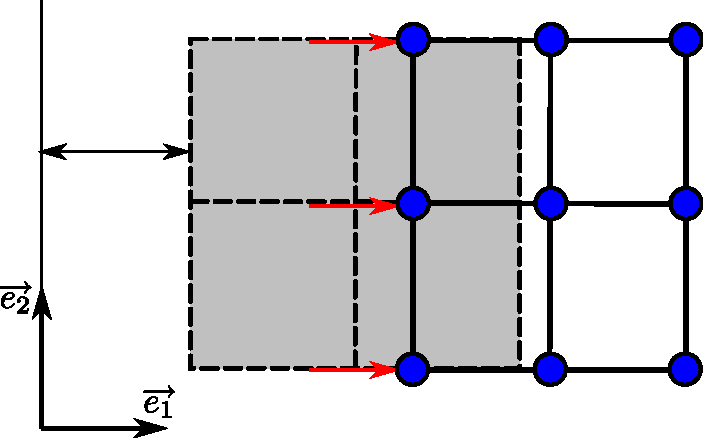
\includegraphics[width=0.5\columnwidth]{Figures/SamplesSingleTorusAbaqus}
\par\end{centering}
\caption{Numerical model for the one element torus test under Abaqus\label{fig:Samples!Single!Torus-Abaqus}}
\end{figure}

\begin{figure}[h]
\begin{centering}
\begin{tabular}{cc}
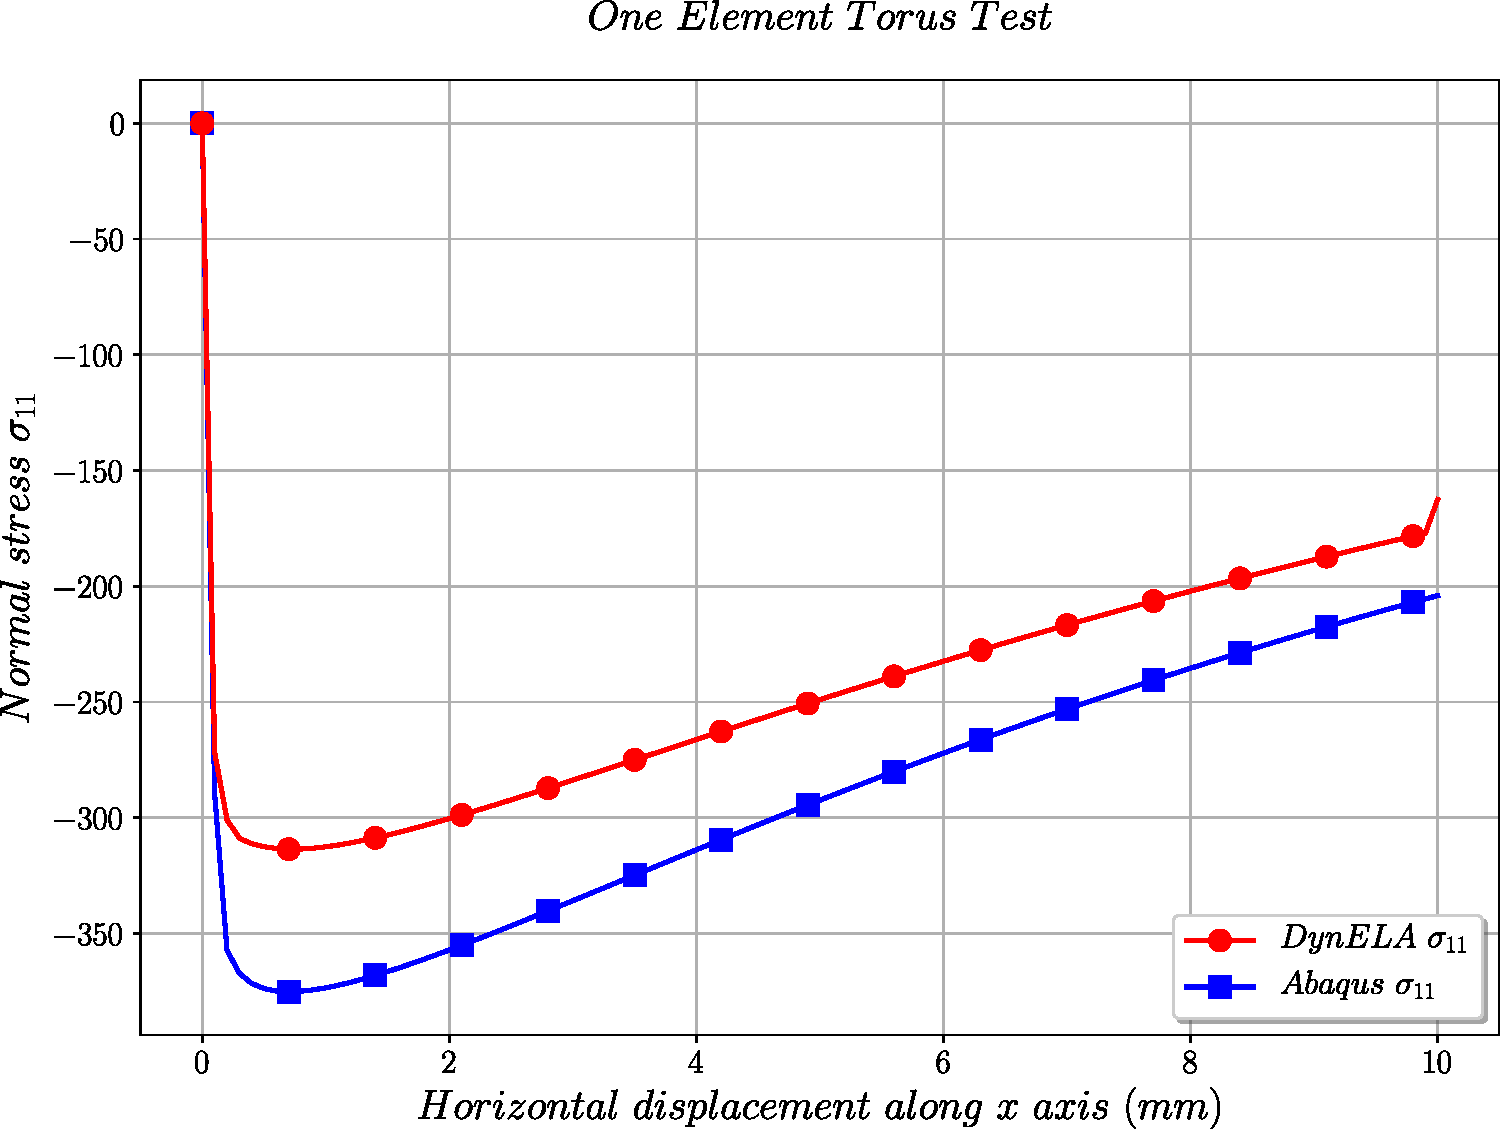
\includegraphics[width=0.45\columnwidth]{Figures/Samples/Element/Torus_stress_11} & 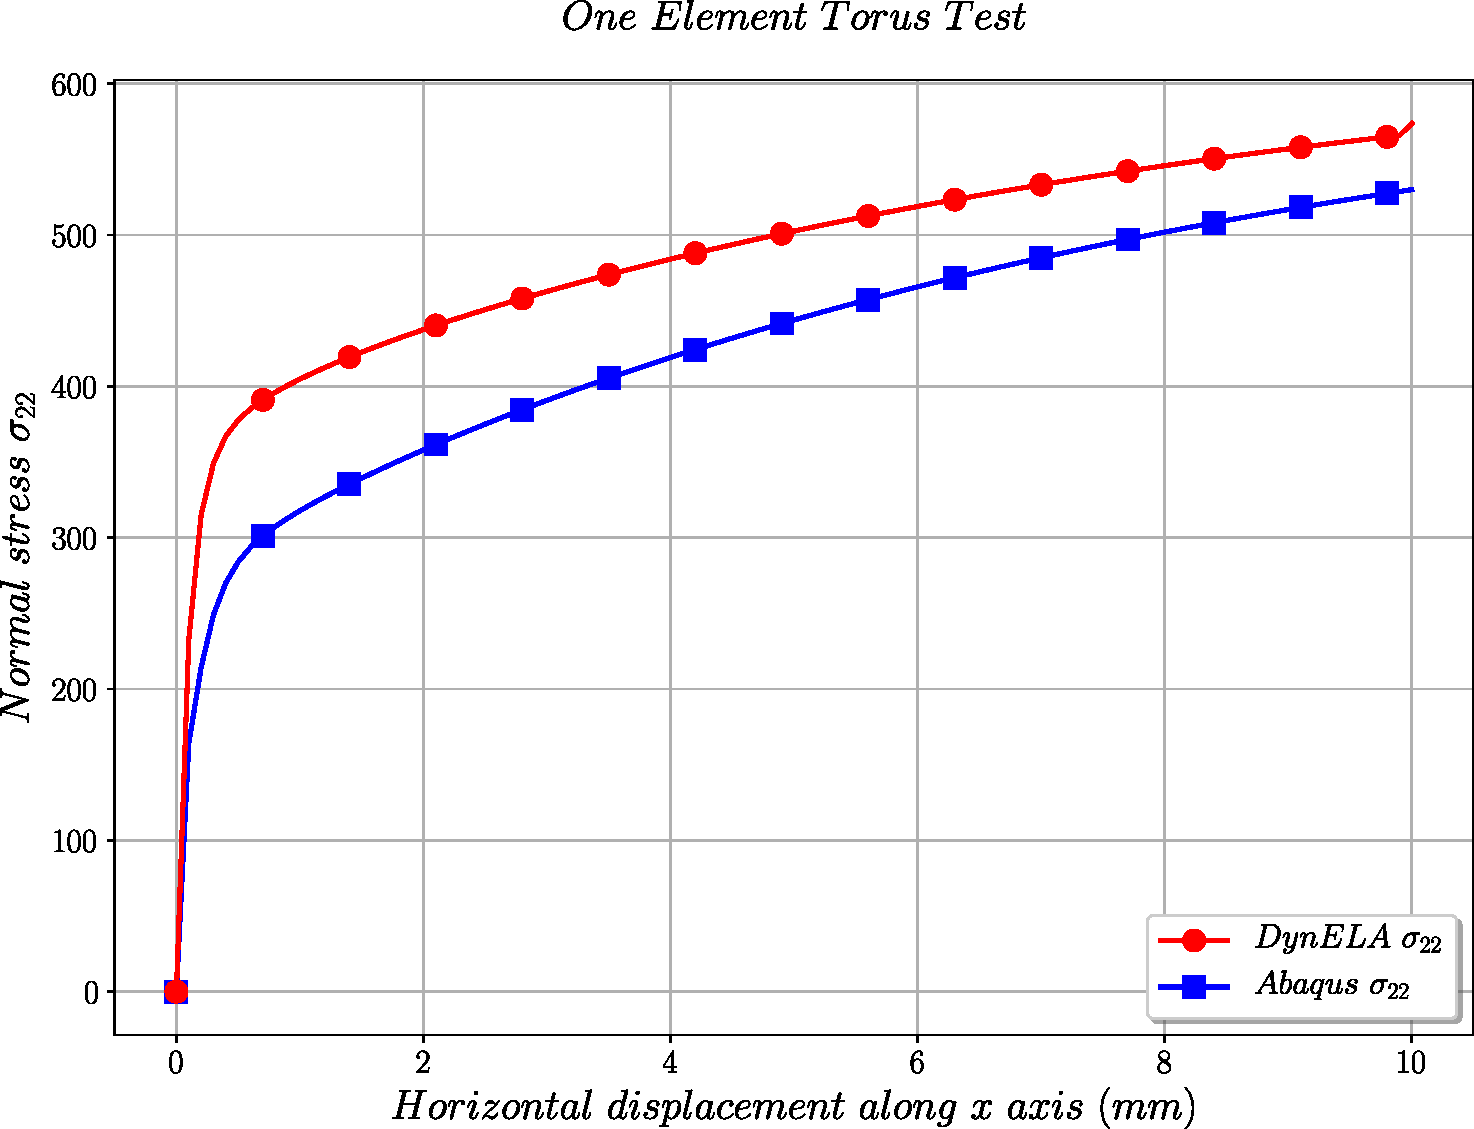
\includegraphics[width=0.45\columnwidth]{Figures/Samples/Element/Torus_stress_22}\tabularnewline
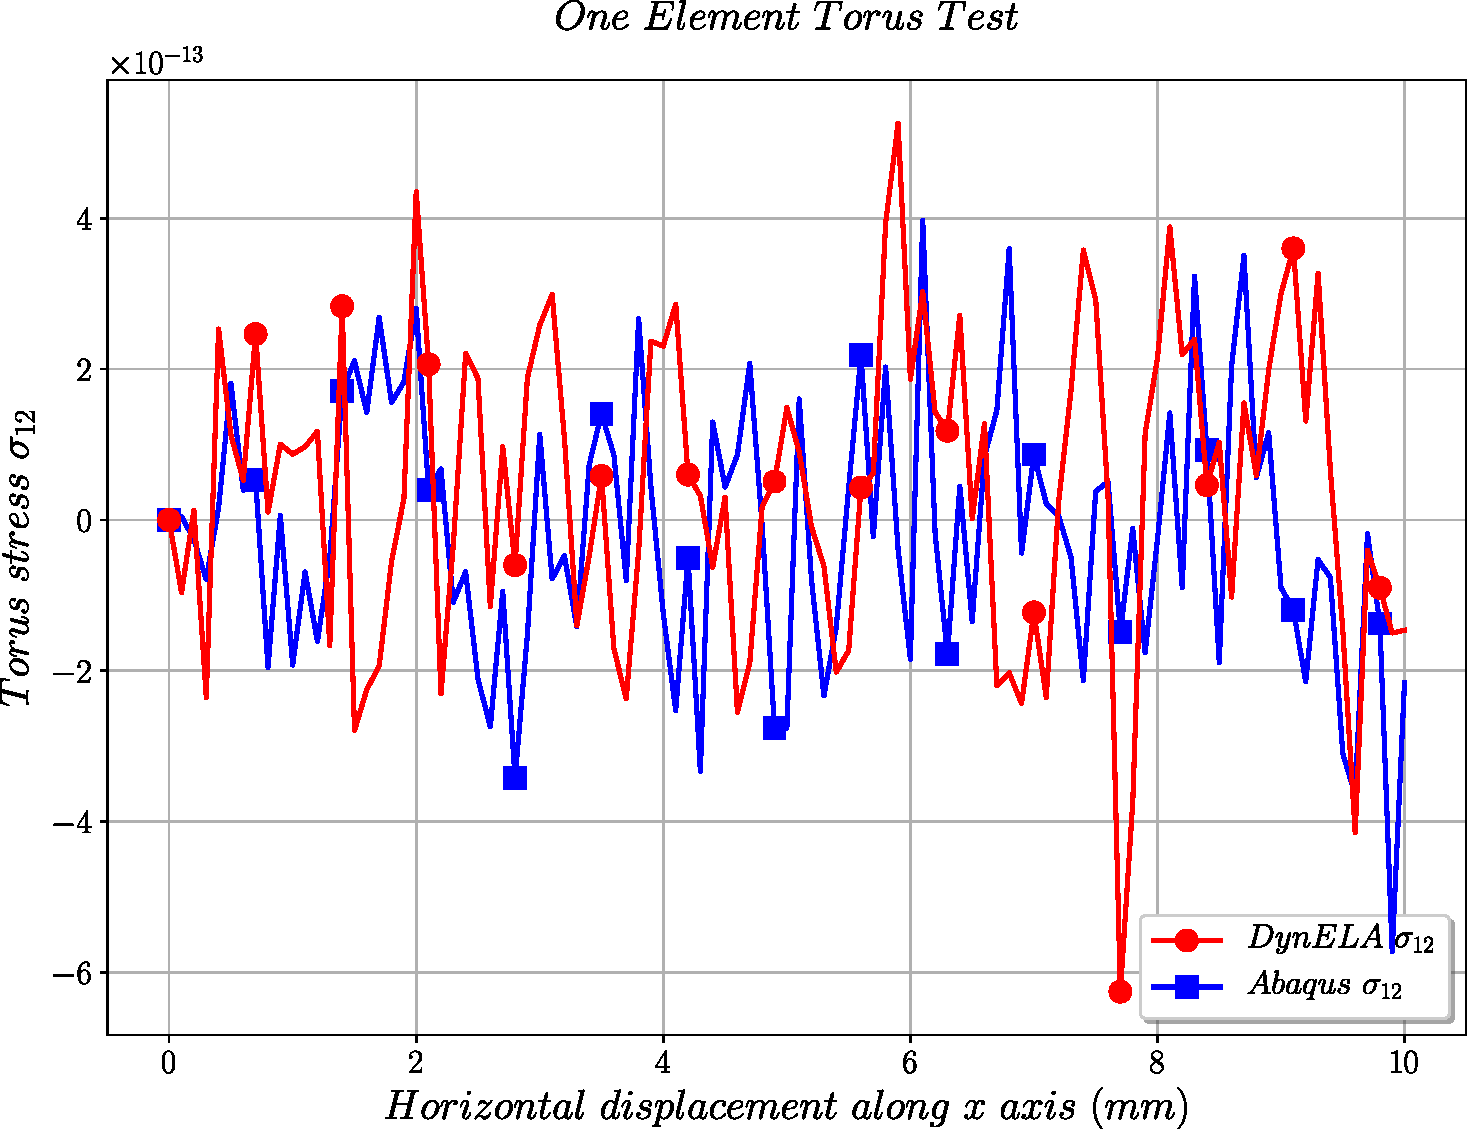
\includegraphics[width=0.45\columnwidth]{Figures/Samples/Element/Torus_stress_12} & 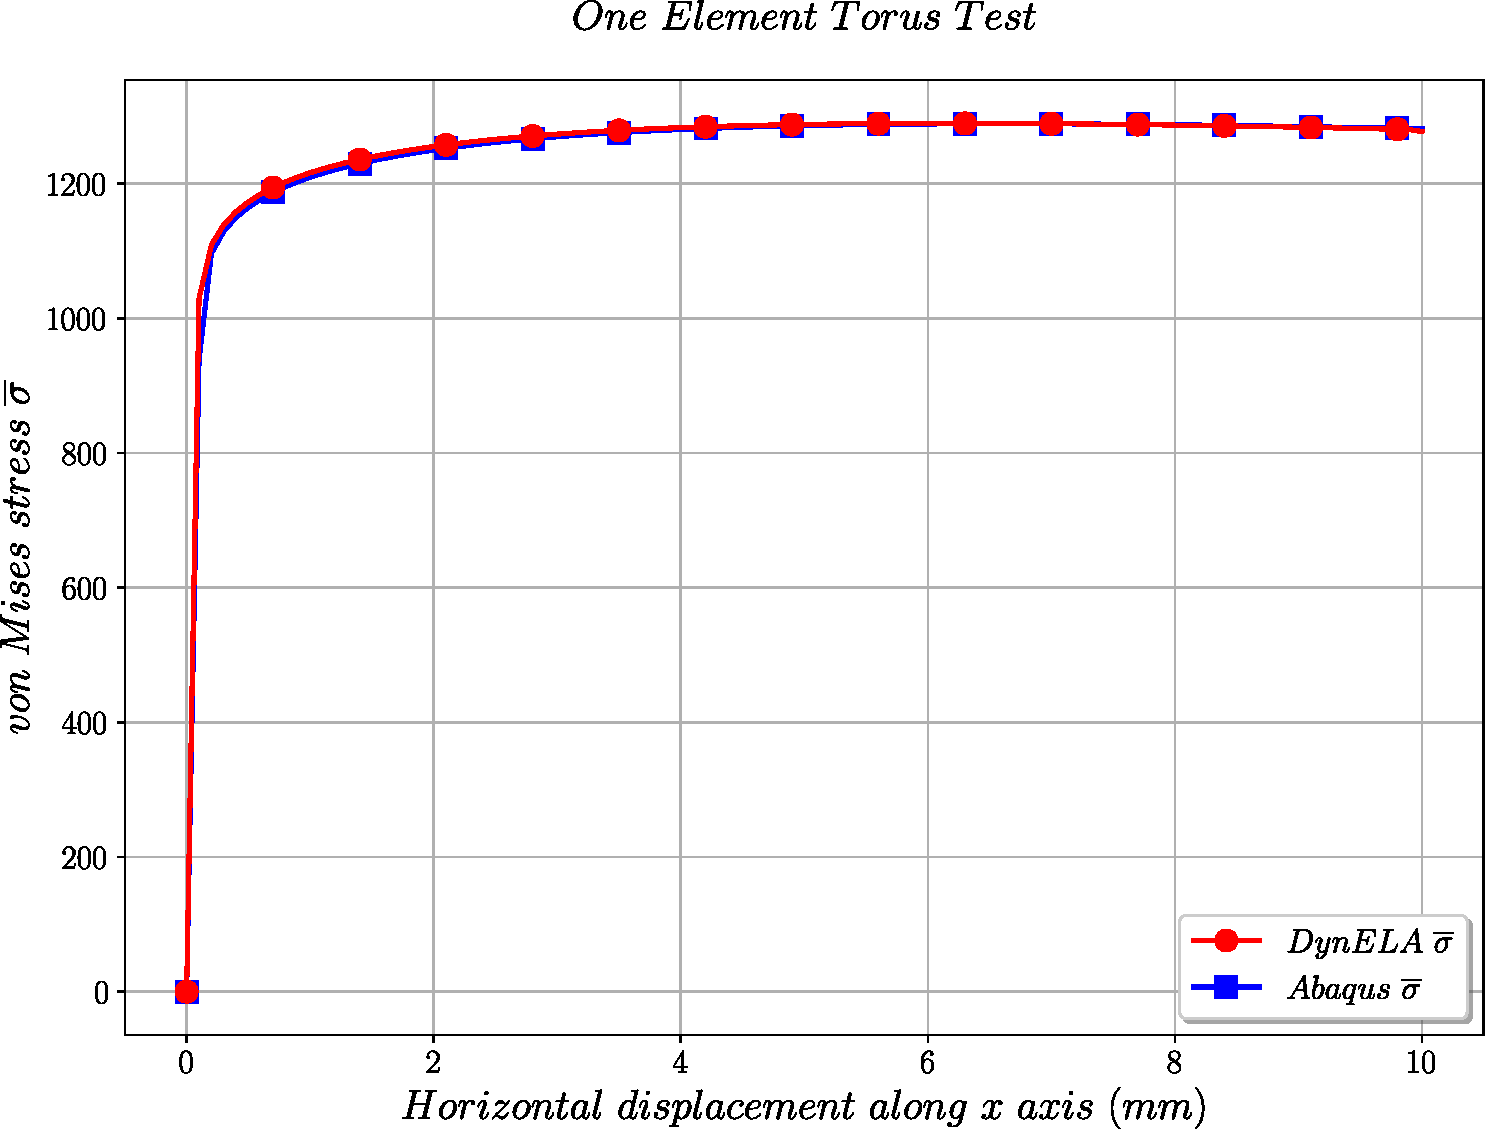
\includegraphics[width=0.45\columnwidth]{Figures/Samples/Element/Torus_vonMises}\tabularnewline
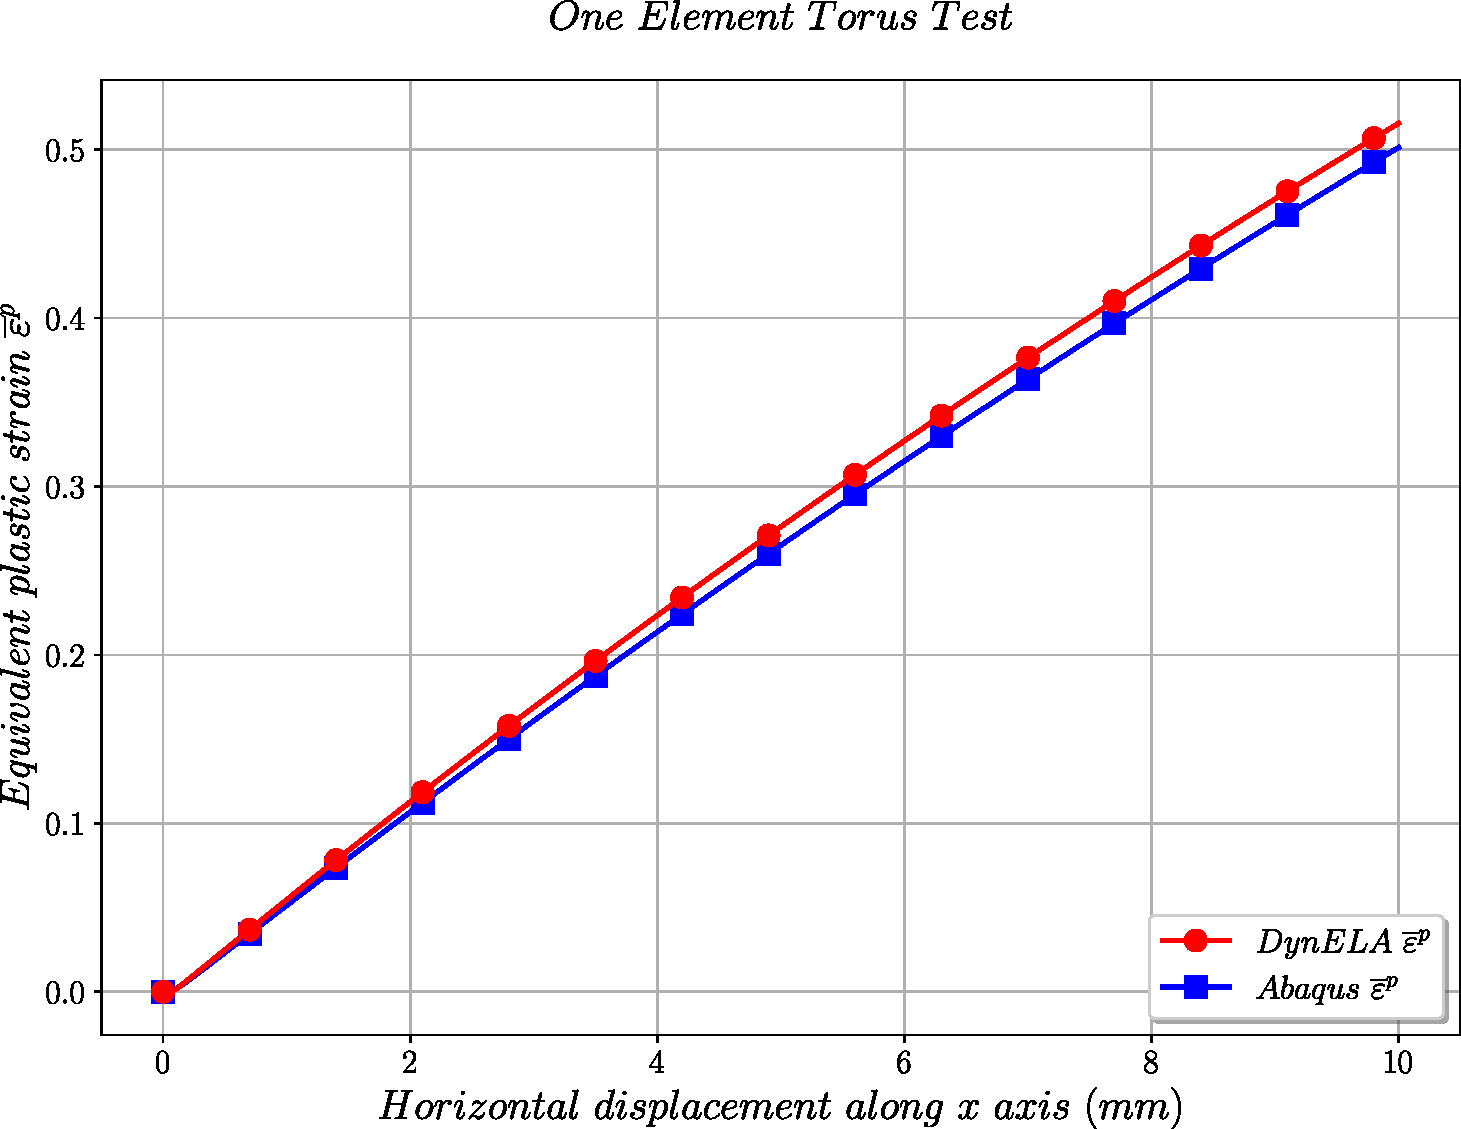
\includegraphics[width=0.45\columnwidth]{Figures/Samples/Element/Torus_plasticStrain} & 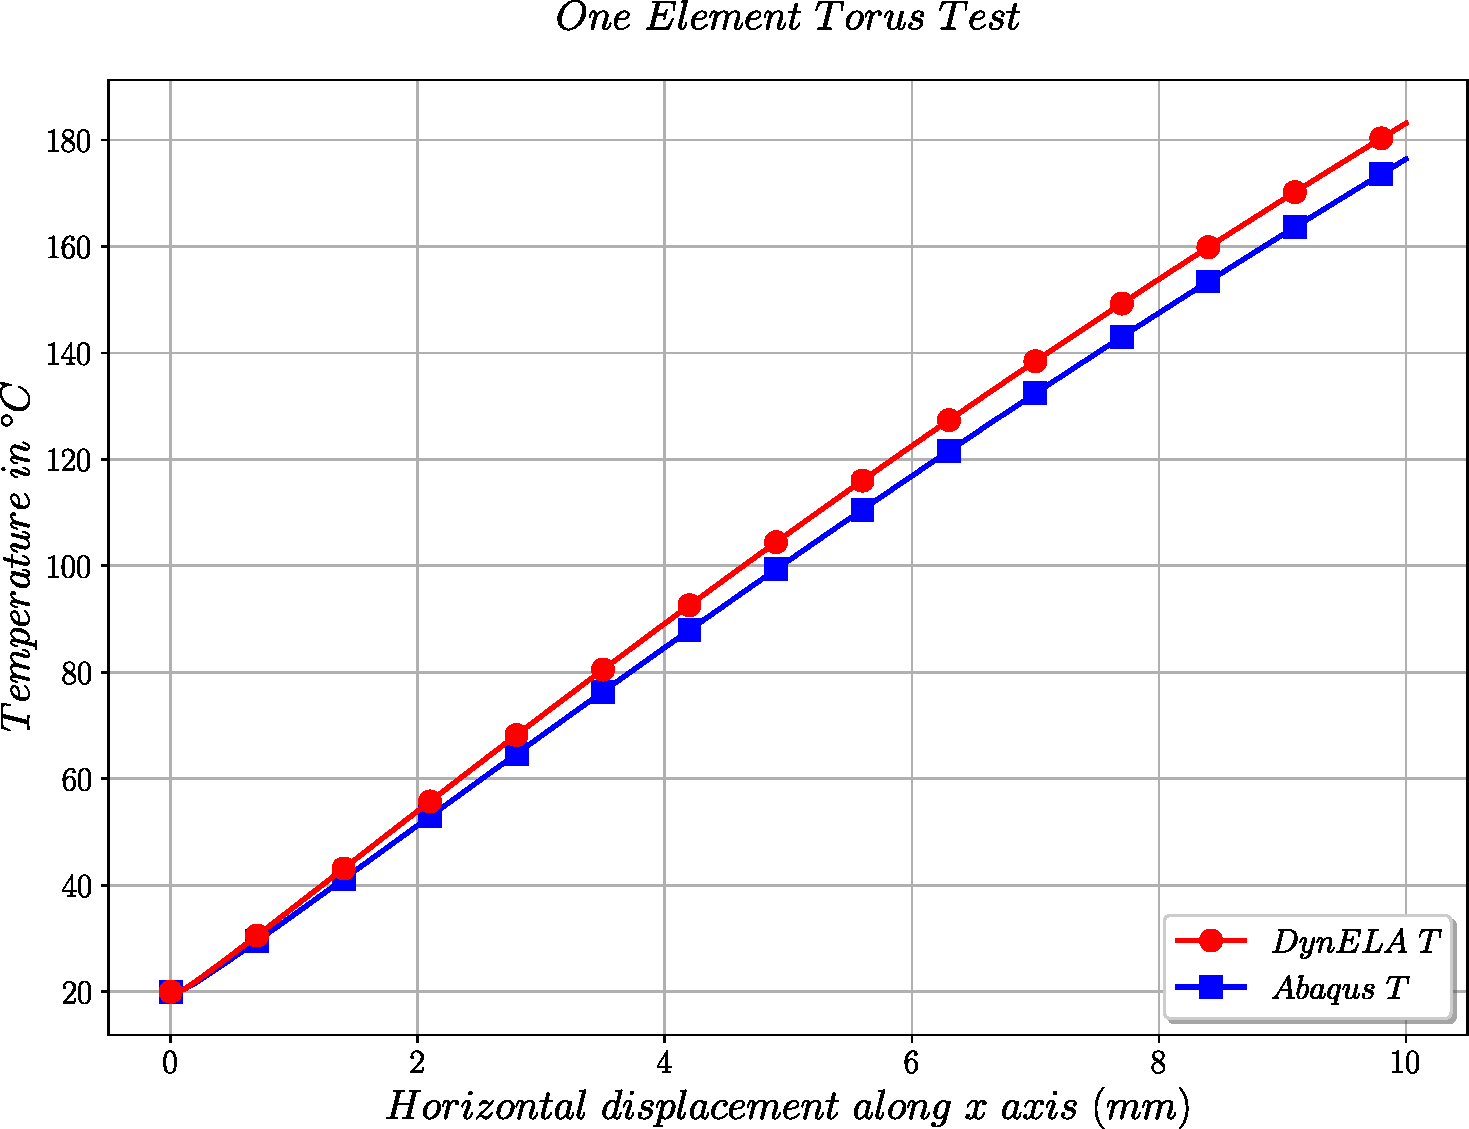
\includegraphics[width=0.45\columnwidth]{Figures/Samples/Element/Torus_temperature}\tabularnewline
\end{tabular}
\par\end{centering}
\caption{Comparison of numerical results for the one element torus tensile
test\label{fig:Samples!Single!Torus-Comparison}}
\end{figure}
\clearpage

\section{Uniaxial one element shear test}

The uniaxial one element shear test is a numerical test where an element
(with a square prescribed shape) is subjected to pure shear test as
presented in figure \ref{fig:Samples!Single!Shear}.
\begin{figure}[h]
\begin{centering}
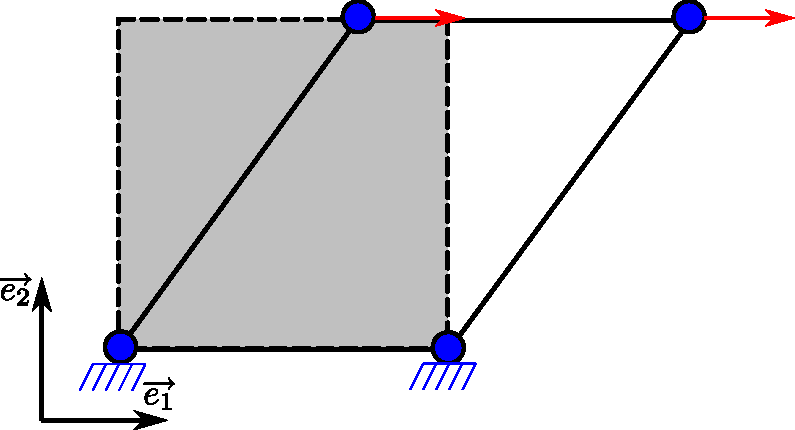
\includegraphics[width=0.5\columnwidth]{Figures/SamplesSingleShear}
\par\end{centering}
\caption{Numerical model for the one element shear test\label{fig:Samples!Single!Shear}}
\end{figure}
 The initial shape of the specimen is $10\,mm\times10\,mm$ and the
the two bottom nodes of the element are encastred and a prescribed
horizontal displacement $d=100\,mm$ is applied on the two upper nodes
of the same element as illustrated in Figure \ref{fig:Samples!Single!Shear}.
As we are using an explicit integration scheme, the total simulation
time is set to $t=0.01\,s$. Mechanical properties of the material
are reported in Table \ref{tab:Samples!JohnsonCookParameters}.

Comparison of Abaqus and DynELA results is made by averaging the DynELA
results on the $4$ integration points of the element. This has been
done because \DynELA~uses full integrated elements while Abaqus
have reduced integrated elements only but in fact, the DynELA results
at the $4$ integration points are the same in this benchmark test.

\subsection{Elastic case}

In this case, only the elastic properties of the constitutive law
reported in Table \ref{tab:Samples!JohnsonCookParameters} are used
and the material is assumed to be hyper-elastic. As we are using a
Jaumann objective rate within the \DynELA, one can obtain, using
an analytical development, the following results for the proposed
case:
\begin{equation}
\Sig=G\left[\begin{array}{ccc}
1-\cos e & \sin e & 0\\
 & \cos e-1 & 0\\
sym &  & 0
\end{array}\right],
\end{equation}
where $G=\mu=\frac{E}{2(1+\nu)}$ is the shear modulus of the material
and $e$ is the elongation along the horizontal axis with $e_{max}=10$
conforming to the prescribed boundaries conditions. Figure \ref{fig:Samples!Single!Shear-Elastic-Comparison}
shows the comparison of the DynELA solver results (plotted in red)
and both the analytical (plotted in blue) and the Abaqus numerical
results (plotted in green) concerning the evolution of the stress
components $\sigma_{11}$, $\sigma_{22}$, $\sigma_{12}$ and $\overline{\sigma}$
\versus  the horizontal displacement of the top edge of the specimen
along the horizontal axis. A perfect match between all those results
can be seen from this later.

\begin{figure}[h]
\begin{centering}
\begin{tabular}{cc}
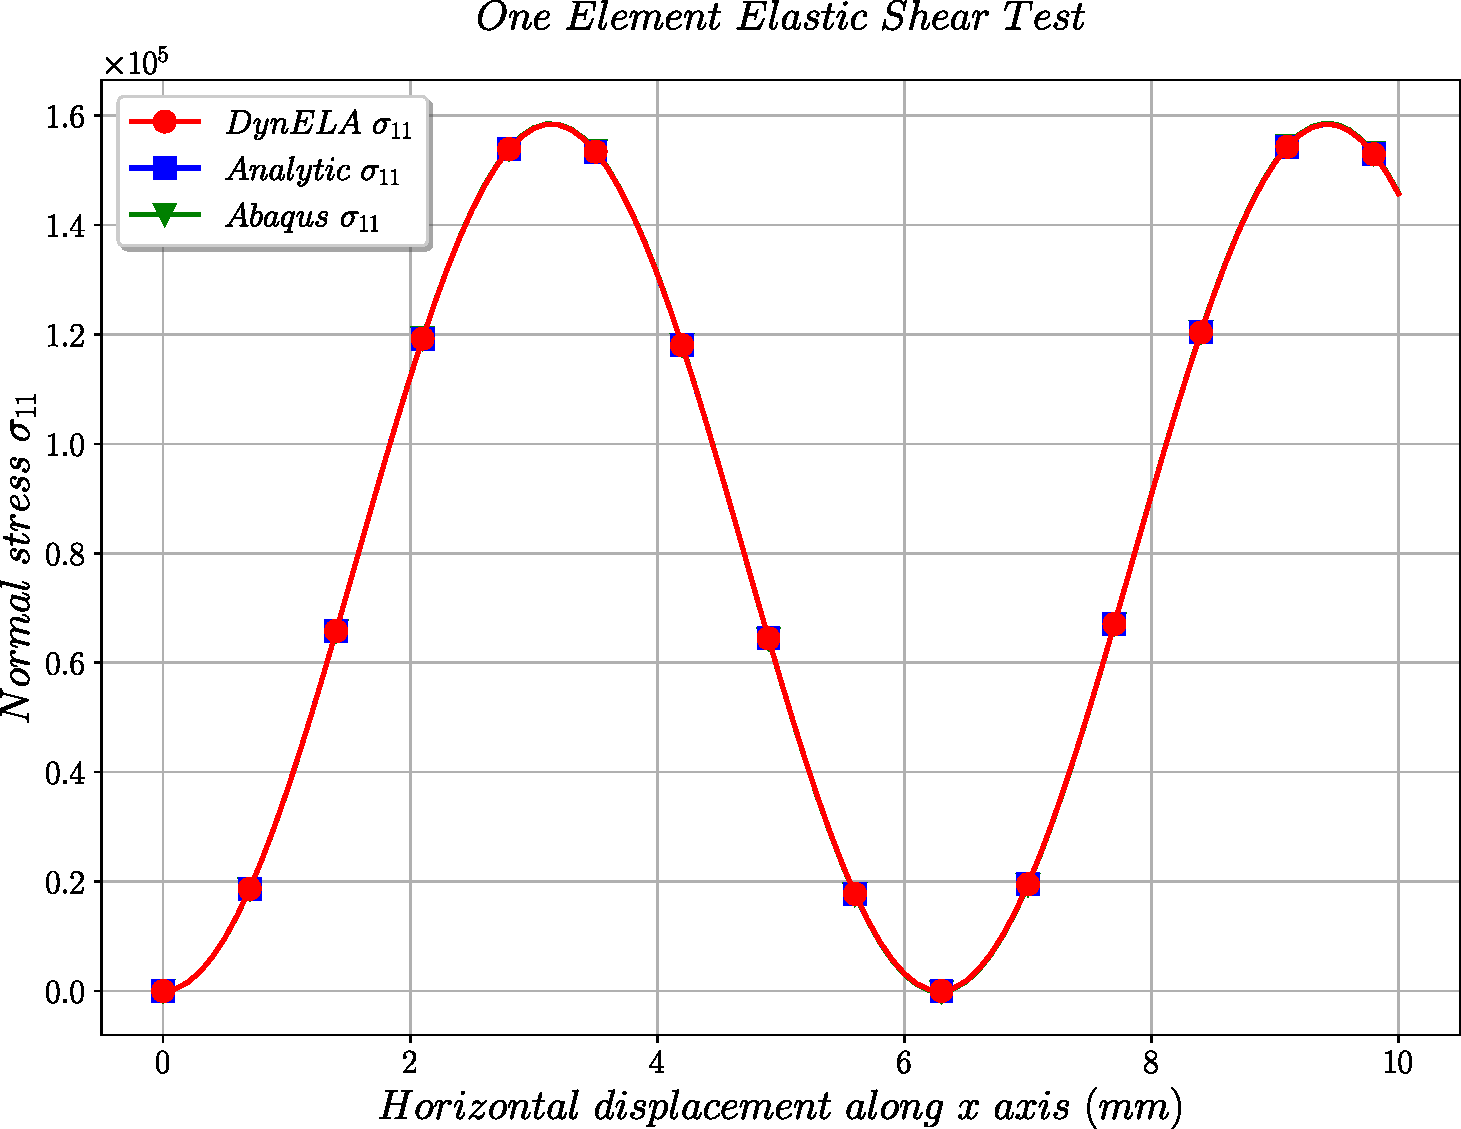
\includegraphics[width=0.45\columnwidth]{Figures/Samples/Element/Shear-Elastic_stress_11} & 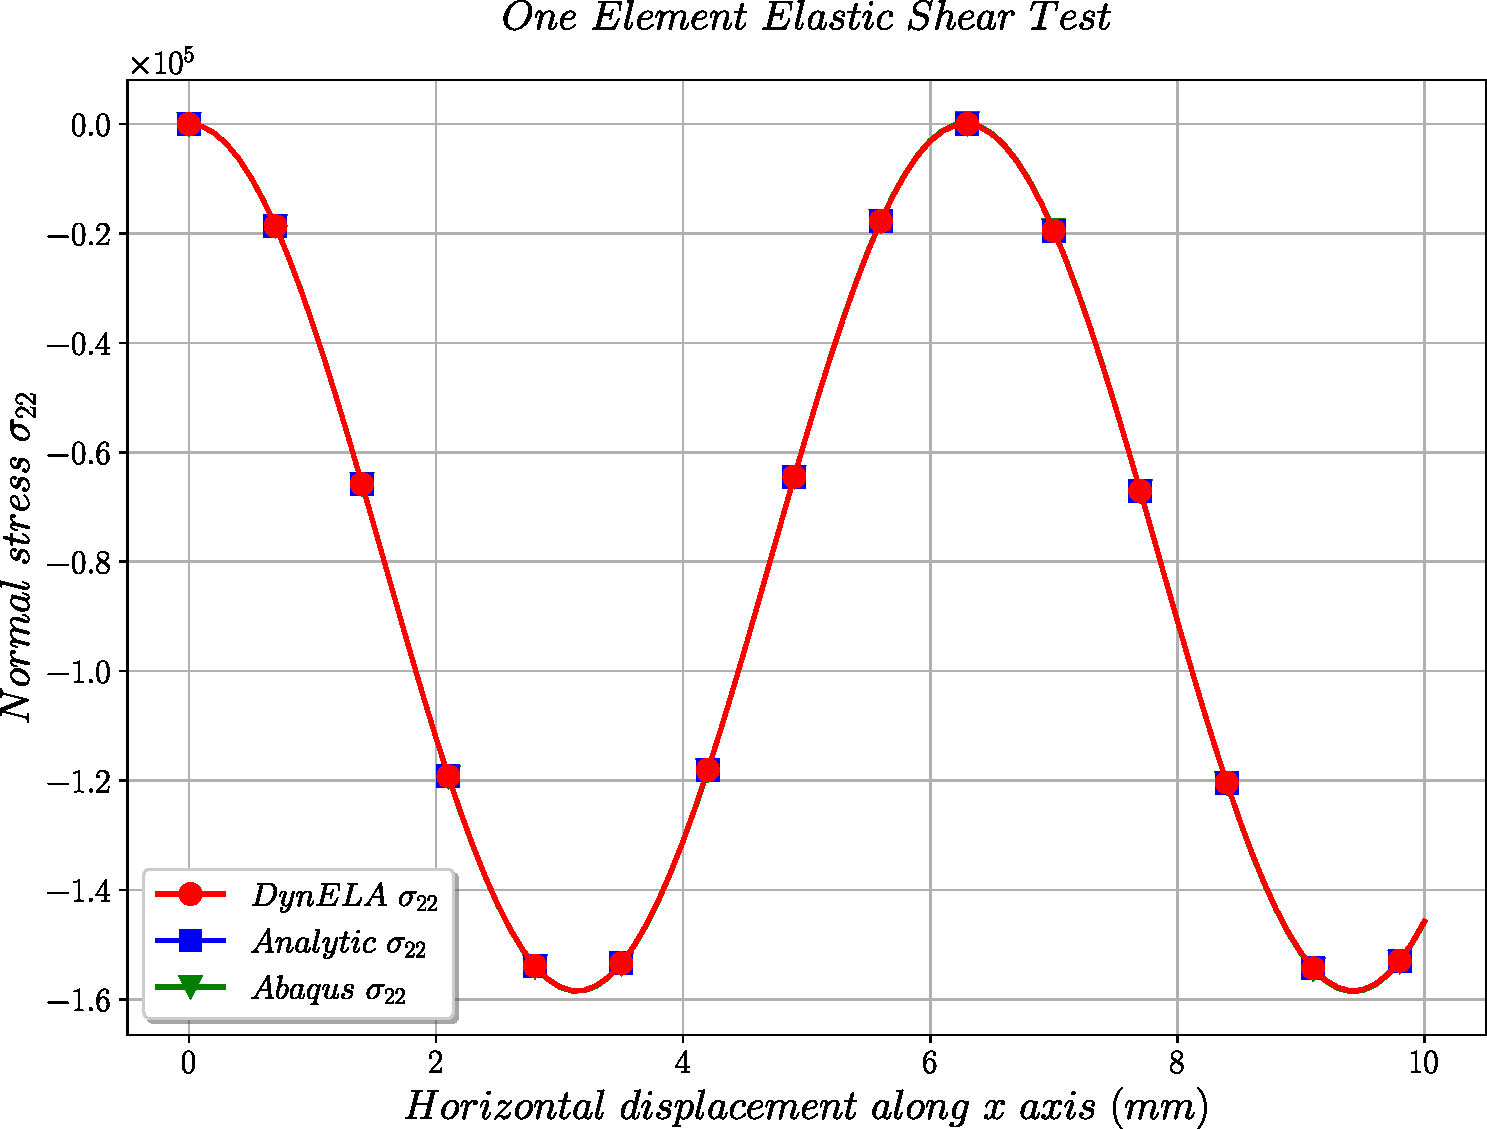
\includegraphics[width=0.45\columnwidth]{Figures/Samples/Element/Shear-Elastic_stress_22}\tabularnewline
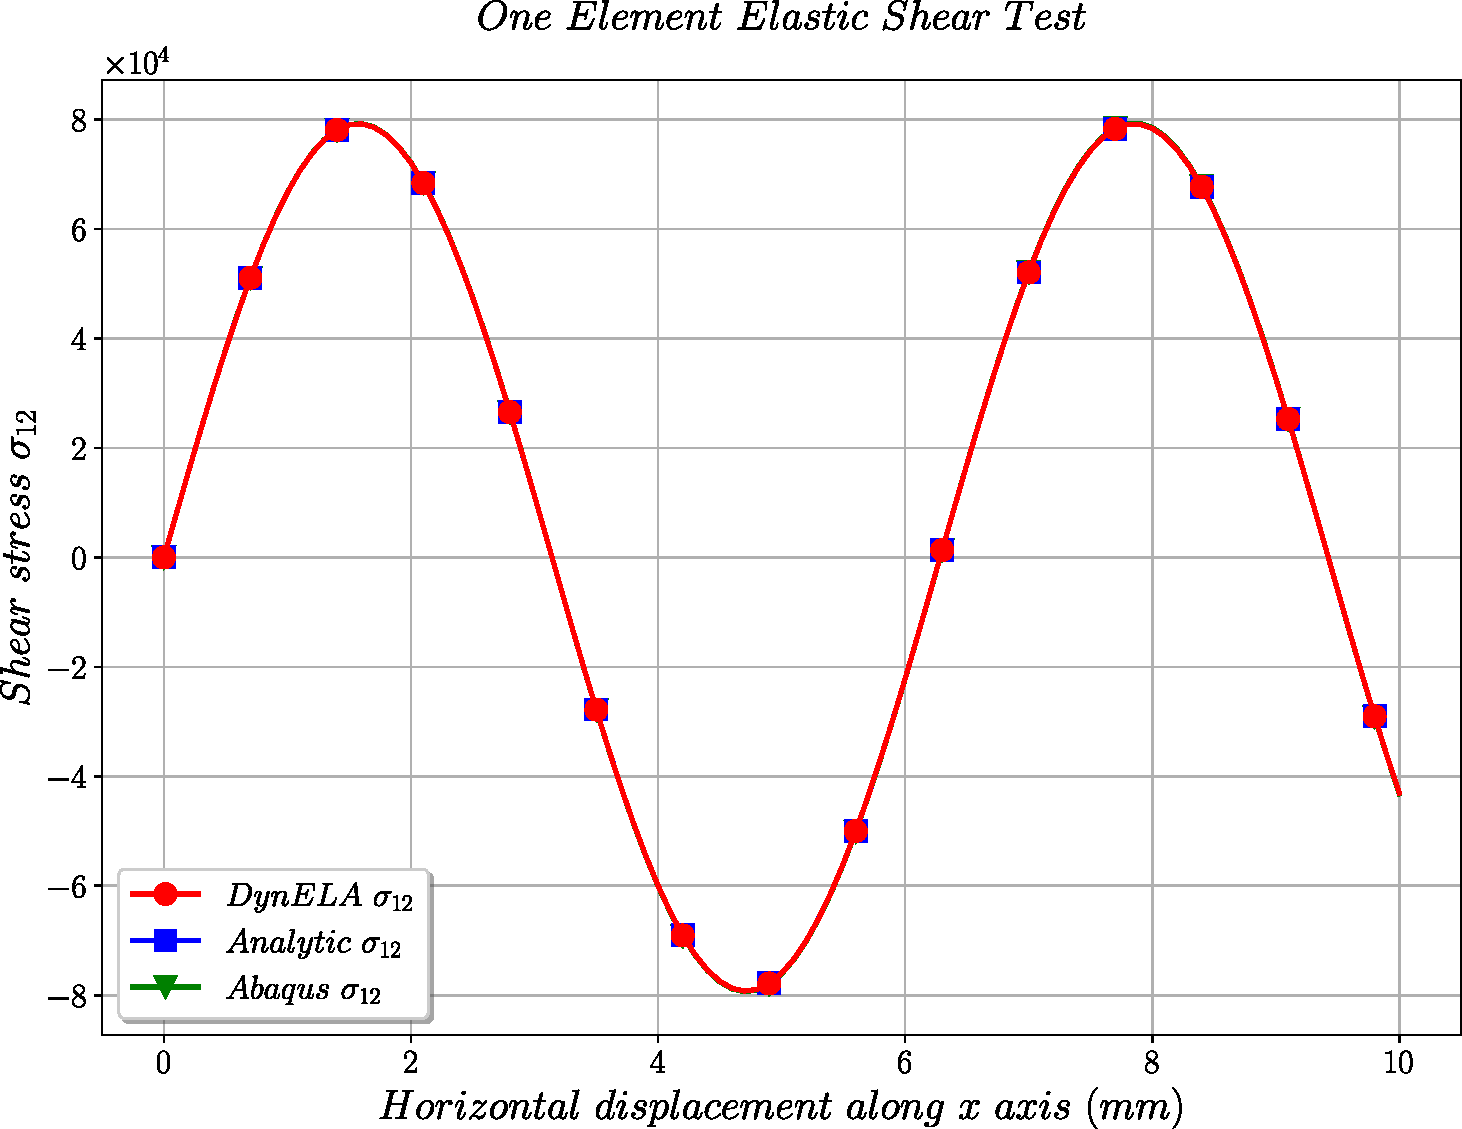
\includegraphics[width=0.45\columnwidth]{Figures/Samples/Element/Shear-Elastic_stress_12} & 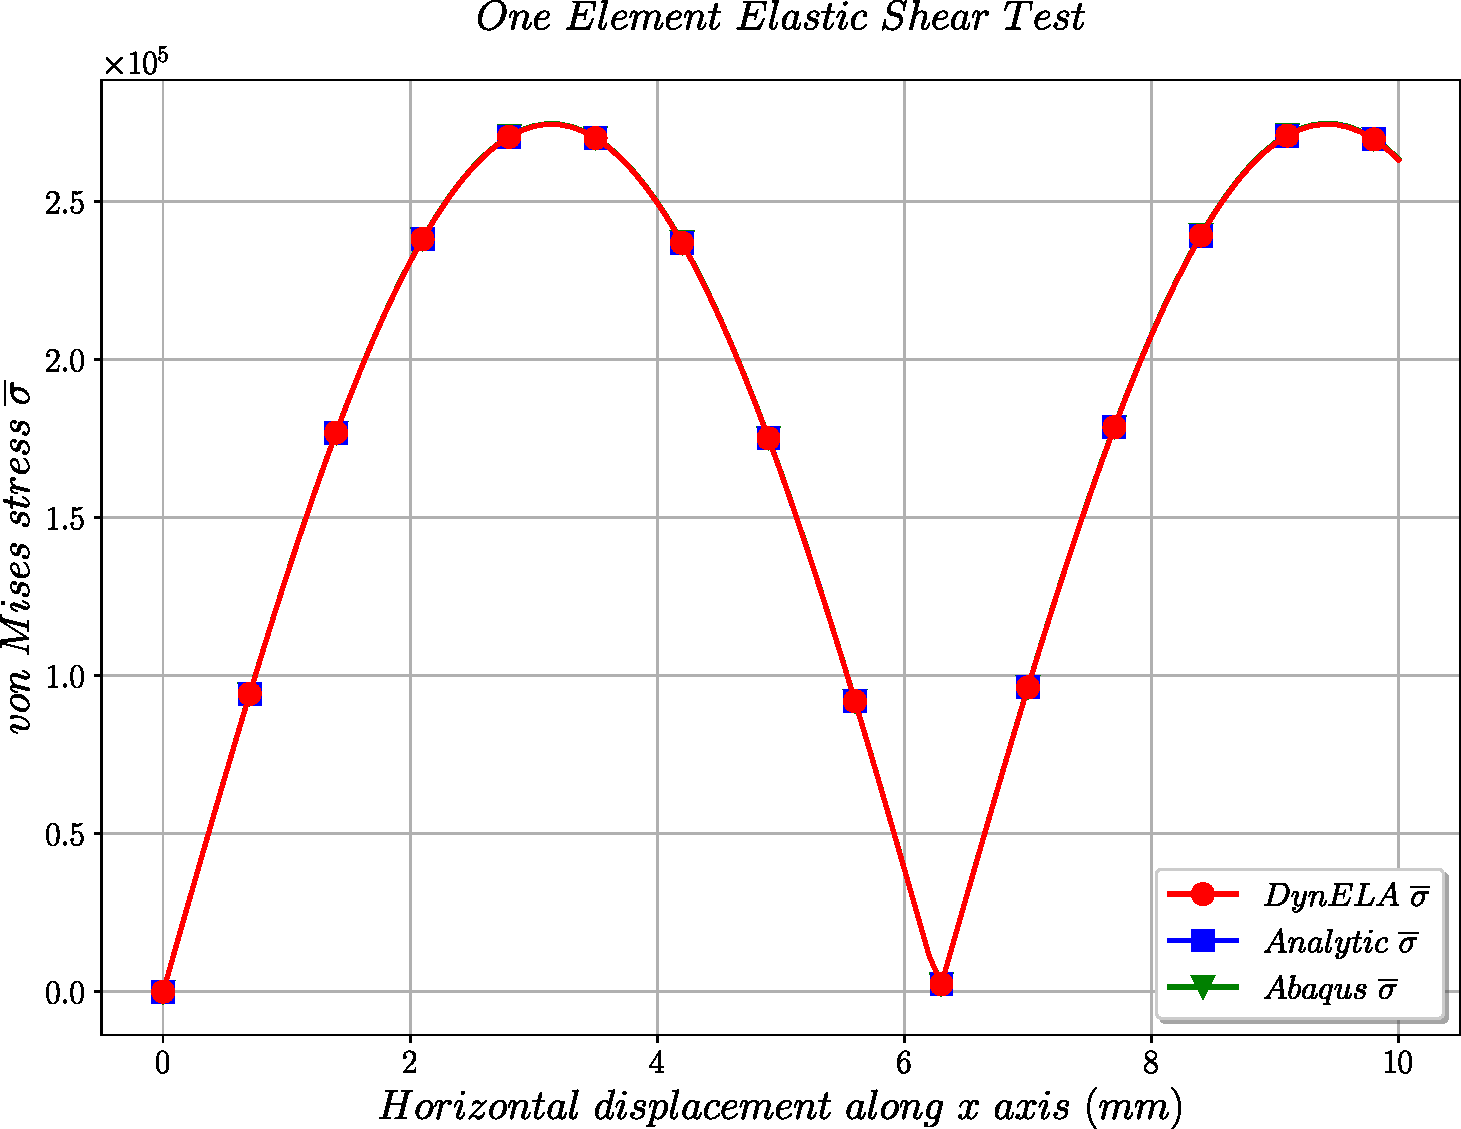
\includegraphics[width=0.45\columnwidth]{Figures/Samples/Element/Shear-Elastic_vonMises}\tabularnewline
\end{tabular}
\par\end{centering}
\caption{Comparison of numerical and analytical results for the one element
elastic shear test\label{fig:Samples!Single!Shear-Elastic-Comparison}}
\end{figure}
\clearpage

\subsection{Johnson-Cook plastic behaviour}

In this case, all the properties of the constitutive law reported
in Table \ref{tab:Samples!JohnsonCookParameters} are used and the
material is assumed to follow the Johnson-Cook behavior described
by equation \ref{eq:Samples!Johnson-Cook}. Figure \ref{fig:Samples!Single!Shear-Comparison}
shows the comparison of the DynELA solver results (plotted in red)
and the Abaqus numerical results (plotted in blue) concerning the
evolution of the stress components $\sigma_{11}$, $\sigma_{22}$,
$\sigma_{12}$, $\overline{\sigma}$, $\overline{\varepsilon}^{p}$
and $T$ \versus  the horizontal displacement of the top edge of
the specimen along the horizontal axis.

\begin{figure}[h]
\begin{centering}
\begin{tabular}{cc}
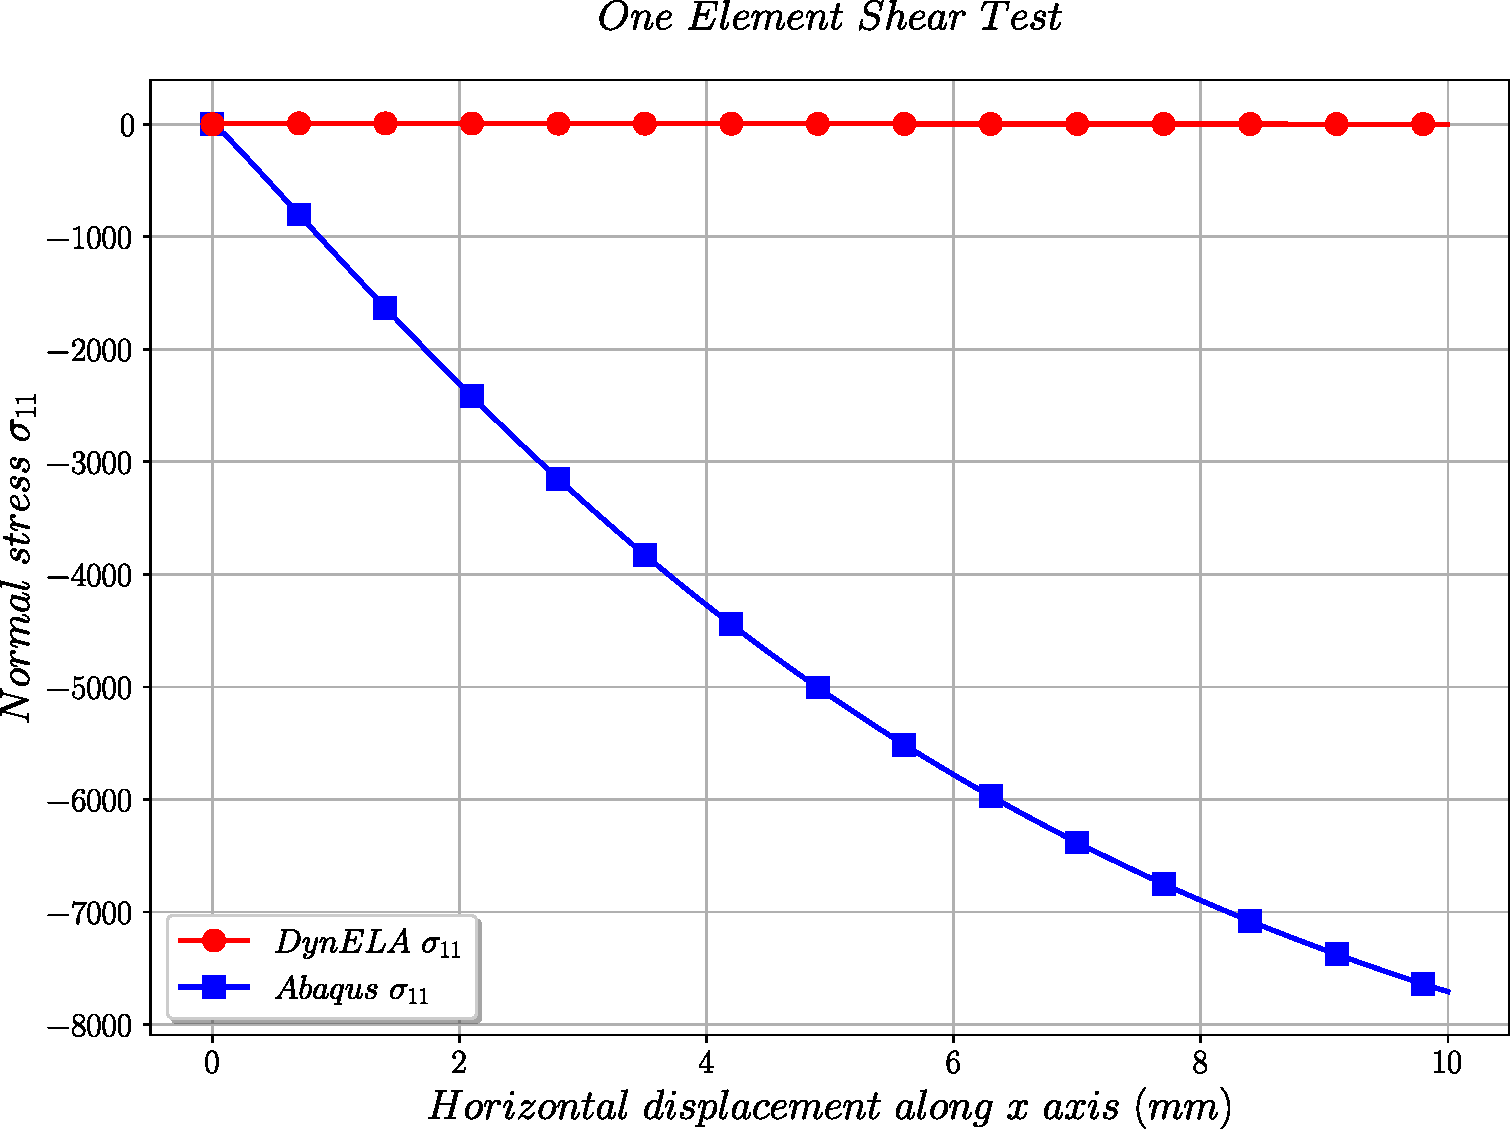
\includegraphics[width=0.45\columnwidth]{Figures/Samples/Element/Shear-Plastic_stress_11} & 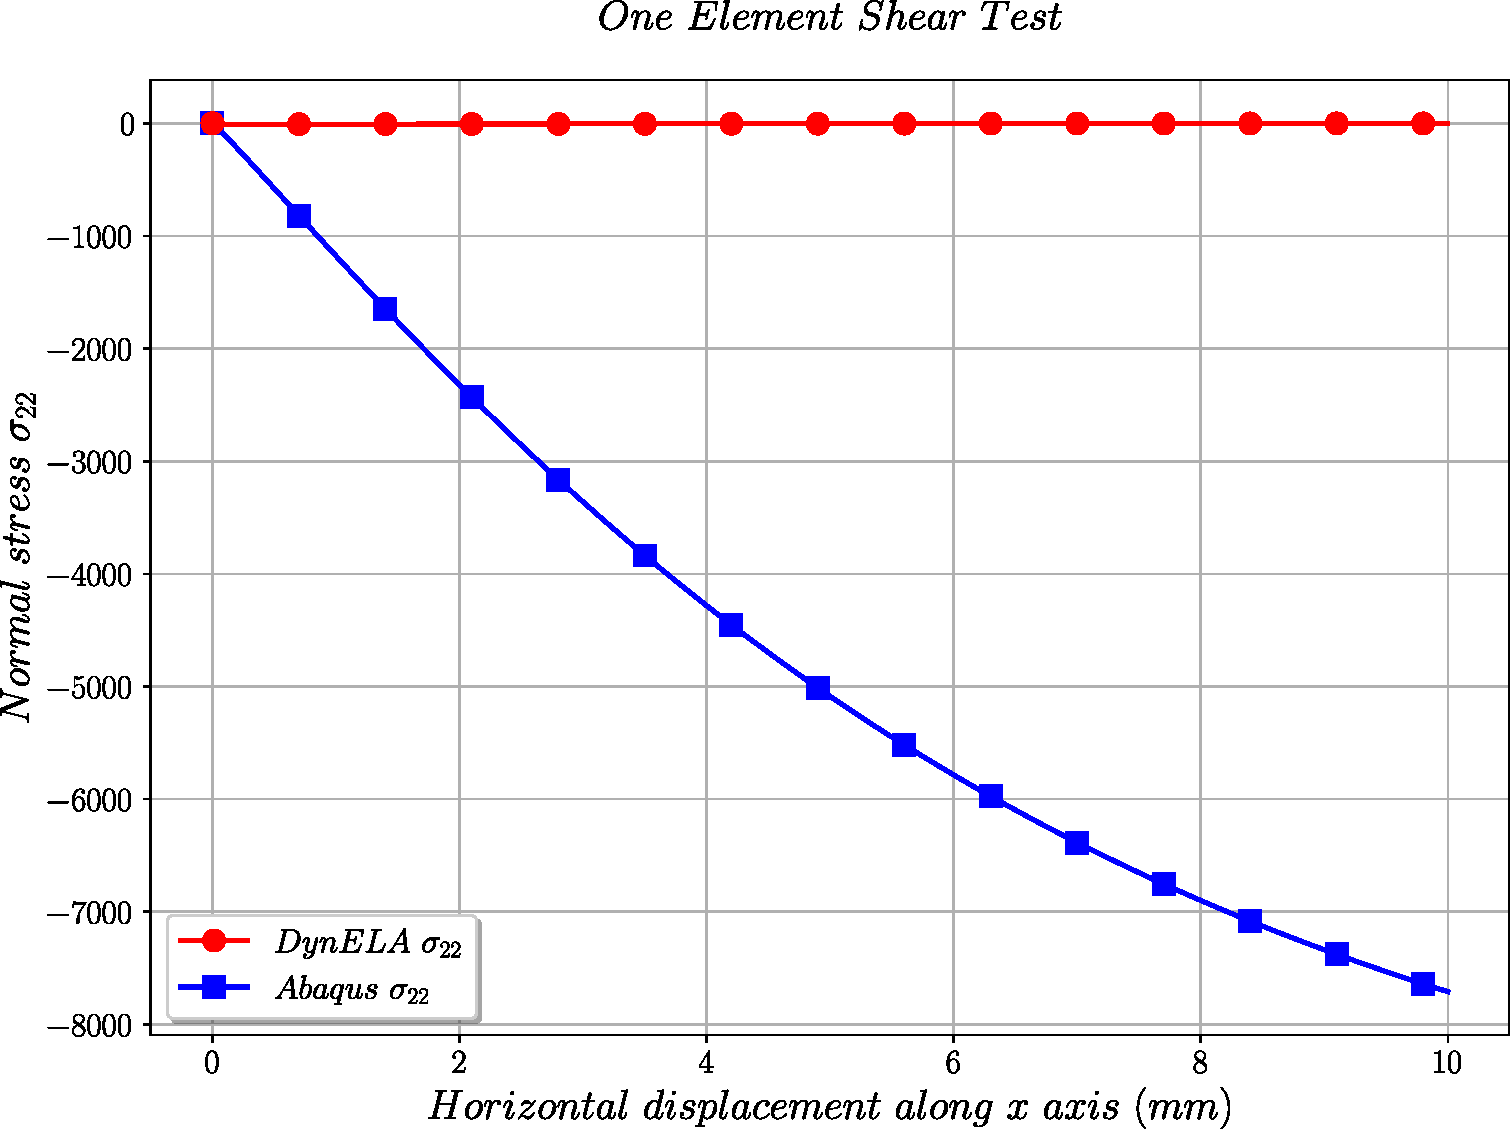
\includegraphics[width=0.45\columnwidth]{Figures/Samples/Element/Shear-Plastic_stress_22}\tabularnewline
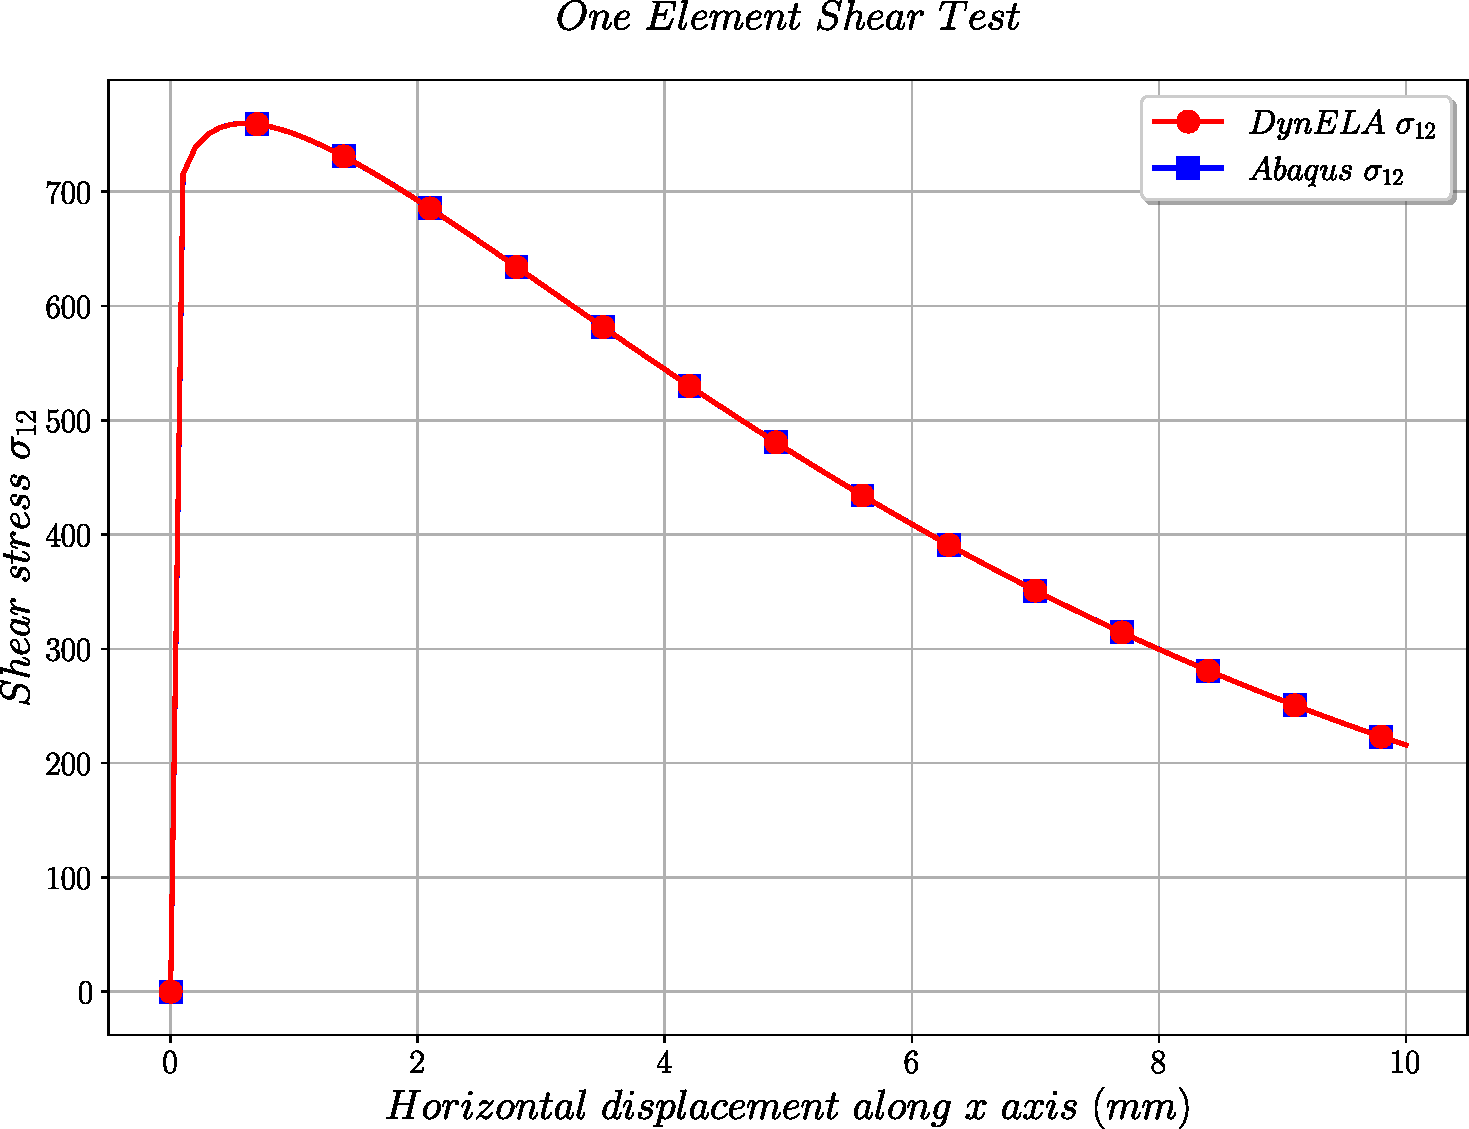
\includegraphics[width=0.45\columnwidth]{Figures/Samples/Element/Shear-Plastic_stress_12} & 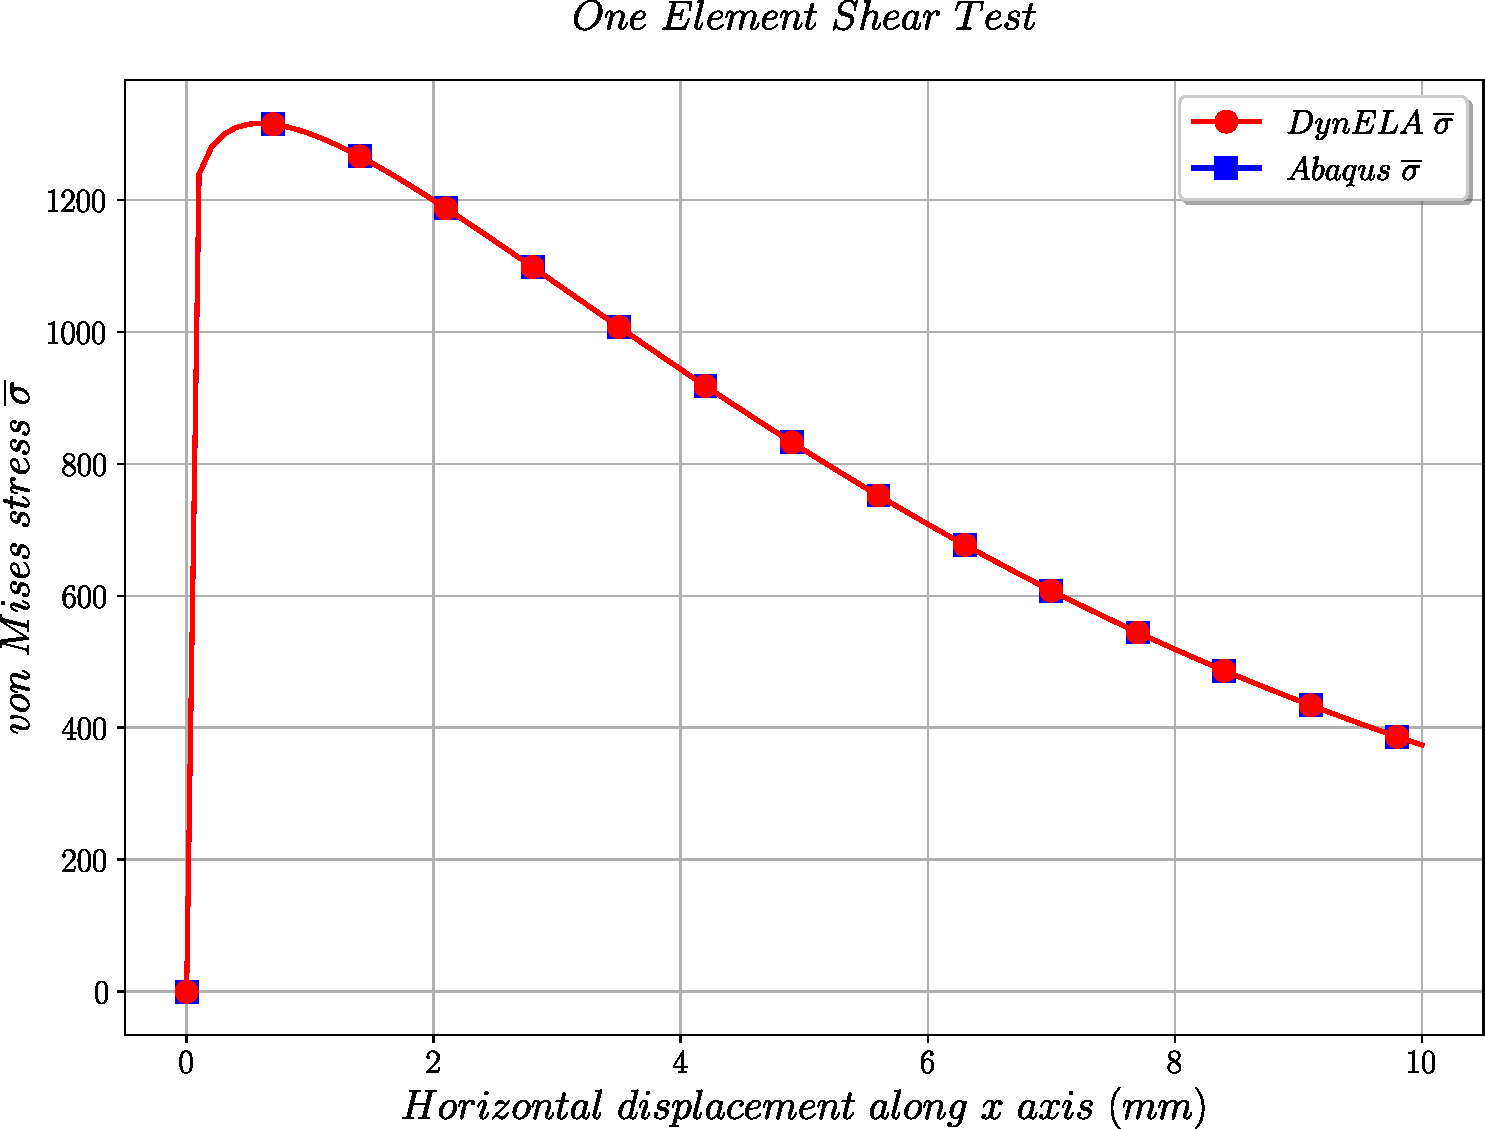
\includegraphics[width=0.45\columnwidth]{Figures/Samples/Element/Shear-Plastic_vonMises}\tabularnewline
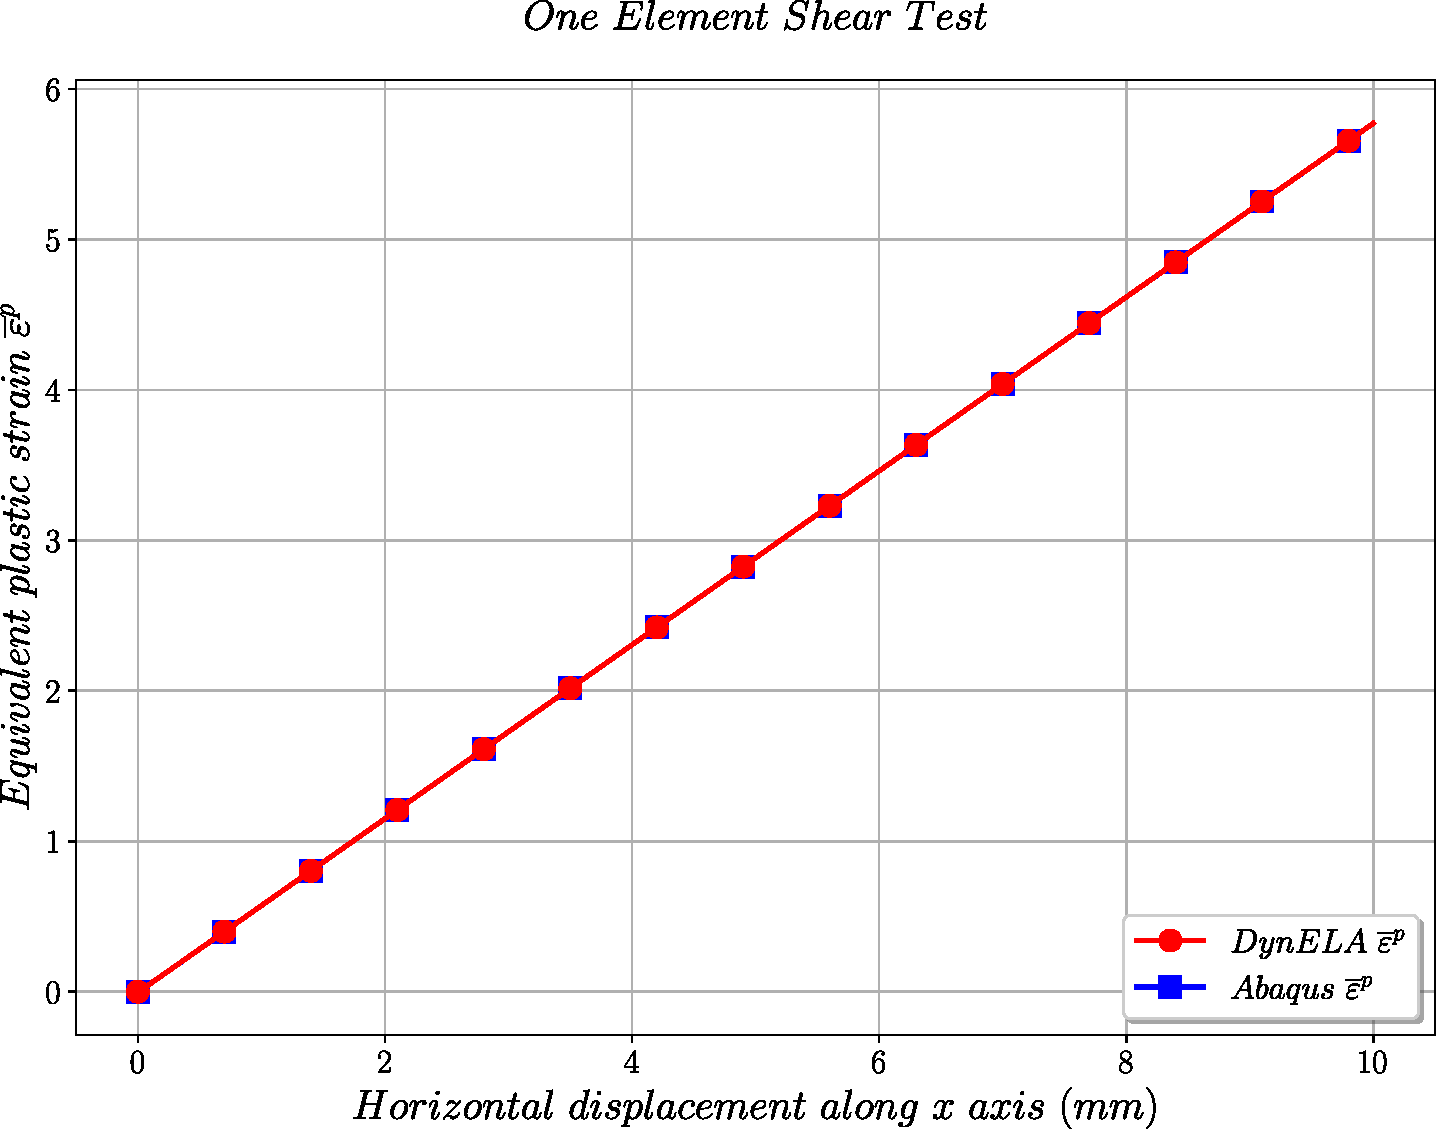
\includegraphics[width=0.45\columnwidth]{Figures/Samples/Element/Shear-Plastic_plasticStrain} & 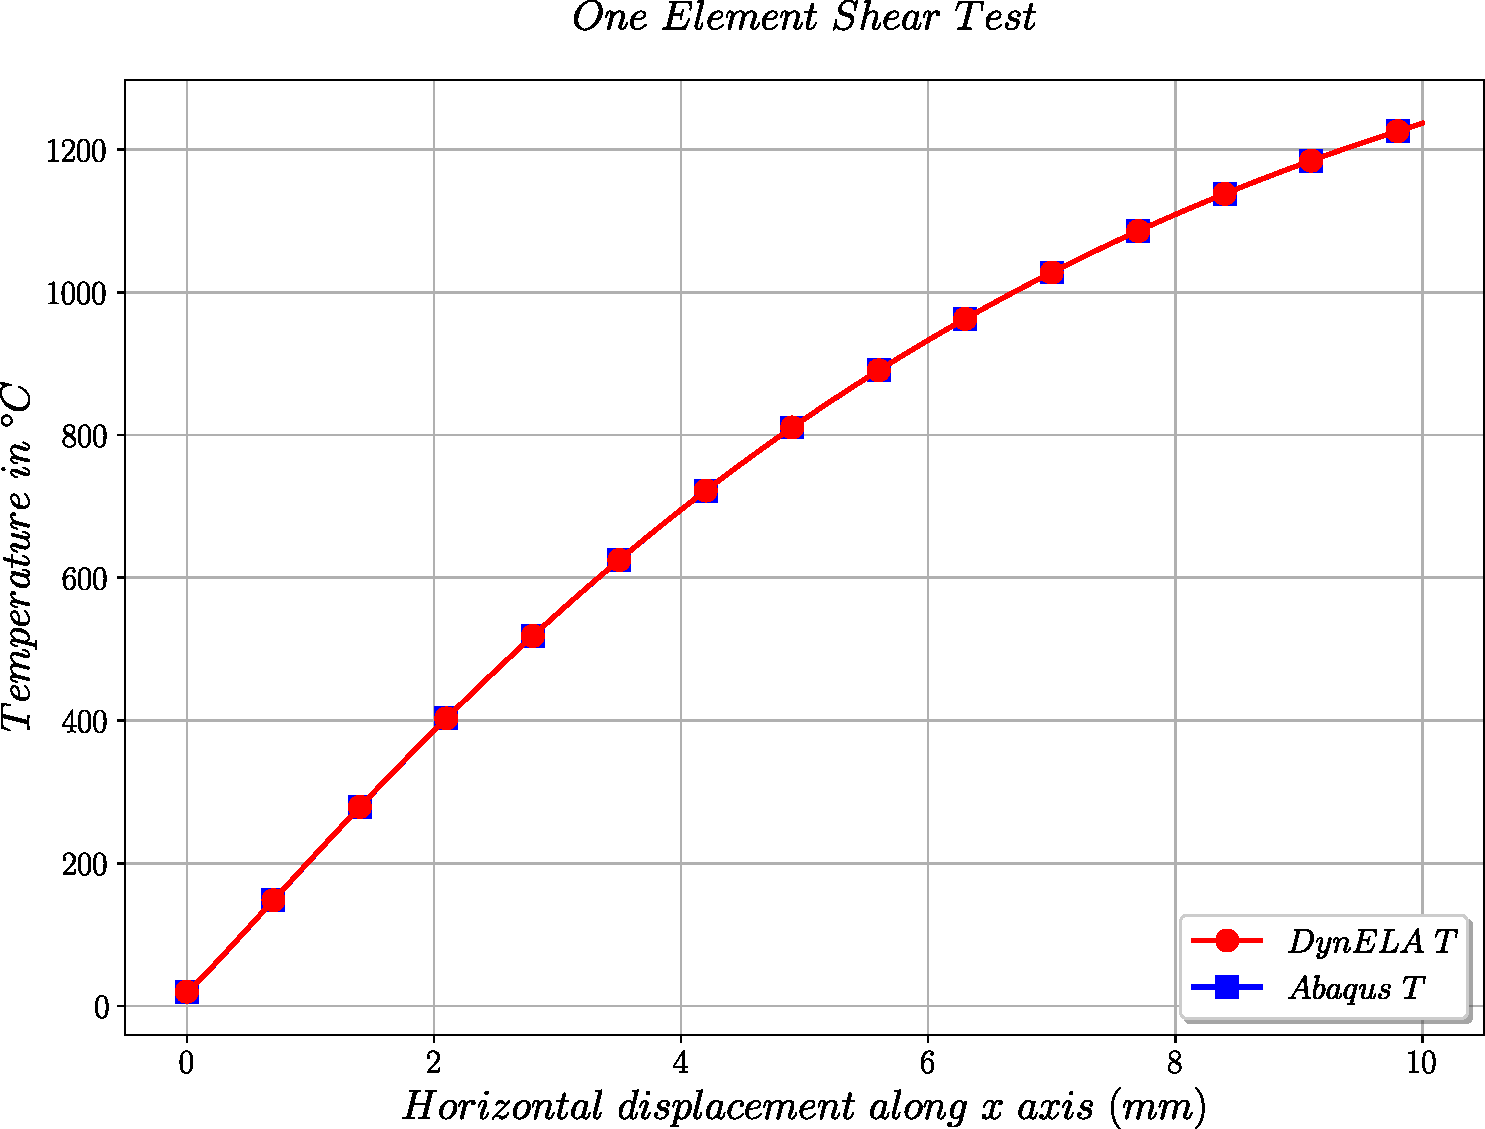
\includegraphics[width=0.45\columnwidth]{Figures/Samples/Element/Shear-Plastic_temperature}\tabularnewline
\end{tabular}
\par\end{centering}
\caption{Comparison of numerical and analytical results for the one element
shear test\label{fig:Samples!Single!Shear-Comparison}}
\end{figure}

